\documentclass[12pt]{article}

\usepackage{algorithm}
\usepackage[noend]{algorithmic}
\usepackage{amsmath}
\usepackage[italian]{babel}
\usepackage{caption}
\usepackage{enumitem}
\usepackage{float}
\usepackage{fullpage}
\usepackage{graphicx}
\usepackage[colorlinks=true, urlcolor=blue]{hyperref}
\usepackage[utf8]{inputenc}
\usepackage{minted}
\usepackage{subcaption}
\usepackage{tabularx}

% Hacks needed to get the algorithm package to work as intended.
\floatname{algorithm}{Algoritmo}
\renewcommand{\algorithmicrequire}{\textbf{Input:}}

\title{Progetto del corso Sistemi Distribuiti: Paradigmi e Modelli, 2012/2013}
\author{
	Jacopo Notarstefano\\
	\texttt{jacopo.notarstefano [at] gmail.com}
}
\date{}

% http://tex.stackexchange.com/a/4304/10806
\newcommand{\cpp}{C\nolinebreak\hspace{-.05em}\raisebox{.4ex}{\tiny\bf +}\nolinebreak\hspace{-.10em}\raisebox{.4ex}{\tiny\bf +}}
\newcommand{\mpp}{Magick\nolinebreak\hspace{-.05em}\raisebox{.4ex}{\tiny\bf +}\nolinebreak\hspace{-.10em}\raisebox{.4ex}{\tiny\bf +}}

\begin{document}
  \maketitle
    \section{Introduzione}

    Scopo di questo progetto è dare un'implementazione sequenziale e una
    parallela di una soluzione al problema dell'Histogram Thresholding, per
    poi confrontarne le performance sia fra esse sia con i modelli teorici.

    Entrambe le implementazioni sono realizzate in \cpp; in particolare
    quella parallela è data in termini di parallel skeleton, più nello
    specifico quelli forniti dal framework 
    \href{http://sketo.ipl-lab.org/}{\underline{SkeTo}}.

    SkeTo è uno skeleton framework in cui dichiarazione e istanziazione degli
    skeleton avvengono allo stesso tempo. I metodi offerti dalle classi
    astratte del framework, implementate in termini di template, sono quelli
    tipici della programmazione funzionale come \texttt{map}, \texttt{reduce}
    e \texttt{scan}. Queste caratteristiche rendono molto compatto il codice:
    in effetti l'intero codice non funzionale parallelo di
    \texttt{src/parallel.cpp} ammonta a \(63\) righe commenti inclusi, di cui
    appena \(3\) chiamate di libreria.

    Il codice non funzionale sequenziale di \texttt{src/sequential.cpp} \`e
    un ordinario programma \cpp. La struttura delle due implementazioni \`e
    molto simile: questo perch\'e il business code dell'applicazione \`e
    stato incapsulato nella classe \texttt{Job}, la cui interfaccia \`e
    definita in \texttt{src/job.h} e la cui implementazione in
    \texttt{src/job.cpp}.

    Per prima cosa presentiamo il problema dell'Histogram Thresholding e
    descriviamo l'algoritmo risolutivo implementato. In seguito descriviamo in
    maggiore dettaglio le scelte implementative adottate durante lo sviluppo.
    Parte centrale del lavoro \`e il confronto delle performance con le
    previsioni teoriche, seguito da una dimostrazione dei risultati ottenuti
    dal programma. Concludiamo con un manuale d'uso che contiene le rule
    definite nel \texttt{Makefile} e gli script disponibili.

    \section{Il problema dell'Histogram Thresholding}

    Siano \texttt{I} un'immagine e \texttt{p} una percentuale. Supponiamo di 
    avere accesso ai singoli pixel dell'immagine, e denotiamo con 
    \texttt{I[i][j]} il pixel alla riga \texttt{i} e colonna \texttt{j}.
    Il problema dell'Histogram Thresholding consiste nel restituire
    un'immagine in bianco e nero \texttt{BW} tale che il pixel
    \texttt{BW[i][j]} sia bianco se il pixel \texttt{I[i][j]} è più luminoso
    di \texttt{p}\% pixel dell'immagine originaria, nero altrimenti.\footnote{
    Osserviamo che in letteratura esistono più definizioni di luminosità di 
    un pixel; le soluzioni proposte usano la coordinata \texttt{L} nello 
    spazio colori \texttt{HSL}.}

    L'algoritmo di risoluzione implementato visita ogni pixel, ne calcola la
    luminosit\`a e la scrive in un vettore. Successivamente lo ordina e
    ricava la luminosit\`a soglia per la percentuale \texttt{p}. Infine visita
    nuovamente ogni pixel dell'immagine originaria e, confrontando con il
    valore soglia precedentemente ottenuto, assegna al corrispondente pixel
    dell'immagine risultante il colore bianco o nero. Pi\`u precisamente
    abbiamo il seguente:

    \begin{algorithm}
      \caption{\textsc{Na\"ive Histogram Thresholding}}
      \begin{algorithmic}[1]
        \REQUIRE \texttt{p} intero, \(0 \le\) \texttt{p} \(< 100\), \texttt{I} immagine di larghezza \texttt{imageWidth} e altezza \texttt{imageHeight}
        \STATE \texttt{luminosities} \(=\) \texttt{[]}
        \FOR{\texttt{i} \(\le\) \texttt{imageWidth}}
          \FOR{\texttt{j} \(\le\) \texttt{imageHeight}}
            \STATE \texttt{luminosities.push(I[i][j].luminosity())}
          \ENDFOR
        \ENDFOR
        \STATE \texttt{luminosities.sort()}
        \STATE \texttt{threshold} \(\leftarrow\) \texttt{luminosities[luminosities.length() * p / 100]}
          \FOR{\texttt{i} \(\le\) \texttt{imageWidth}}
            \FOR{\texttt{j} \(\le\) \texttt{imageHeight}}
              \IF{\texttt{I[i][j].luminosity()} \(>\) \texttt{threshold}}
                \STATE \texttt{BW[i][j]} \(\leftarrow\) \texttt{white}
              \ELSE
                \STATE \texttt{BW[i][j]} \(\leftarrow\) \texttt{black}
              \ENDIF
            \ENDFOR
          \ENDFOR
          \RETURN \texttt{BW}
        \end{algorithmic}
    \end{algorithm}

    \section{Descrizione delle implementazioni}

    Abbiamo posto particolare enfasi nella divisione fra codice funzionale e
    non funzionale; in particolare il business code dell'applicazione è
    interamente astratto nella classe \texttt{Job}.

    Osserviamo che i metodi \texttt{execute} e \texttt{writeResult} hanno
    come tipo di ritorno \texttt{Job}; in effetti questi metodi ritornano
    l'oggetto stesso. Ciò consente di usarli in \texttt{sequential.cpp} come
    se avessero tipo di ritorno \texttt{void}, cio\`e ignorandone il valore
    di ritorno, e in \texttt{parallel.cpp} come argomento di
    \texttt{generate} e \texttt{map}. \`E necessario astrarli in opportuni
    function object, ad esempio:

    \inputminted[]{c++}{tex/src/function-object.cpp}

    Come gi\`a detto l'implementazione parallela usa SkeTo, in particolare la
    versione \texttt{1.1}. Esiste una versione pi\`u aggiornata, la
    \texttt{1.50pre}, scartata perch\'e ad oggi priva di documentazione.
    Internamente SkeTo si avvale di un'implementazione disponibile di MPI;
    quella utilizzata da questo progetto \`e la distribuzione
    \href{http://www.mpich.org}{\underline{MPICH}} versione \texttt{3.0.4}. 
    La lettura e scrittura delle immagini sono interamente delegate alla
    libreria \href{http://www.imagemagick.org/script/index.php}{\underline{ImageMagick}}
    tramite \href{http://www.imagemagick.org/script/magick++.php}{\underline{\mpp}},
    la sua API per \cpp, versione \texttt{6.8.6-9}. Usiamo infine la libreria \href{http://www.libpng.org/pub/png/libpng.html}{\underline{libpng}} versione \texttt{1.6.3} per la manipolazione di immagini in formato \texttt{png}.

    \section{Valutazione delle performance}

    Entrambe le implementazioni sono state eseguite sia su una macchina con
    pi\`u core sia su un cluster di pi\`u macchine. In questa sezione
    riportiamo i risultati e li confrontiamo con i modelli teorici.

    Analizzando il codice \`e facile rendersi conto che il problema da
    risolvere \`e parallelo sui dati. Ci aspettiamo quindi che il tempo di
    servizio decresca linearmente con il numero di elementi di calcolo
    impiegati.

    \subsection{Multicore}

    I seguenti test sono stati svolti su \texttt{andromeda.di.unipi.it},
    macchina con 2 processori Intel Xeon E5520 a 4 core con clock a 2.27GHz,
    ciascuno dotato di 2 contesti. 
    
    Ci aspettiamo quindi uno speedup quasi lineare fino a 8 elementi di
    calcolo, in seguito un plateau delle performance e un calo
    dell'efficienza.

    Siano \(T_{\text{seq}}\) e \(T_{\text{par}}(n)\) rispettivamente il 
    service time dell'applicazione sequenziale e di quella parallela con
    grado di parallelismo \(n\). L'esecuzione degli script
    \texttt{awk/service\_time.awk} e \texttt{awk/multicore\_service\_time.awk}
    permette di stimare \(T_{\text{seq}} \approx 1.12\) e \(T_{\text{par}}(n)\)
    come dalla seguente tabella:

    \begin{table}[H]
      \begin{tabularx}{\linewidth}{{c}l*{16}{X}}
        \(n\) & 1 &  2 &  3 &  4 &  5 &  6 &  7 &  8
              & 9 & 10 & 11 & 12 & 13 & 14 & 15 & 16 \\
        \hline
        \(T_{\text{par}}(n)\) & 1.15 & .55 & .39 & .28 & .23 & .20 & .17 & .15
                        & .15 & .15 & .15 & .15 & .14 & .16 & .14 & .15 \\
      \end{tabularx}
    \end{table}

    L'esecuzione dello script \texttt{awk/multicore\_speedup.awk}
    permette di stimare lo speedup \(s(n)\) come segue:

    \begin{table}[H]
      \begin{tabularx}{\linewidth}{{c}l*{16}{X}}
        \(n\) & 1 &  2 &  3 &  4 &  5 &  6 &  7 &  8
              & 9 & 10 & 11 & 12 & 13 & 14 & 15 & 16 \\
        \hline
        \(s(n)\) & 0.98 & 2.03 & 2.98 & 4.03 & 4.95 & 5.65 & 6.50 & 7.43
                 & 7.44 & 7.65 & 7.42 & 7.25 & 7.80 & 7.21 & 7.99 & 7.49 \\
      \end{tabularx}
    \end{table}

    Dallo script \texttt{awk/multicore\_scalability.awk} ricaviamo le
    seguenti stime per la scalabilità \(\text{scalab}(n)\):

    \begin{table}[H]
      \begin{tabularx}{\linewidth}{{c}l*{16}{X}}
        \(n\) & 1 &  2 &  3 &  4 &  5 &  6 &  7 &  8
              & 9 & 10 & 11 & 12 & 13 & 14 & 15 & 16 \\
        \hline
        \(\text{scalab}(n)\) & 1.00 & 2.08 & 2.96 & 4.13 & 5.07 & 5.79 & 6.66 & 7.62
                 & 7.63 & 7.84 & 7.60 & 7.43 & 7.99 & 7.39 & 8.19 & 7.67 \\
      \end{tabularx}
    \end{table}

    Inoltre dallo script \texttt{awk/multicore\_efficiency.awk}
    possiamo stimare l'efficienza \(\epsilon(n)\) come in tabella:

    \begin{table}[H]
      \begin{tabularx}{\linewidth}{{c}l*{16}{X}}
        \(n\) & 1 &  2 &  3 &  4 &  5 &  6 &  7 &  8
              & 9 & 10 & 11 & 12 & 13 & 14 & 15 & 16 \\
        \hline
        \(\epsilon(n)\) & .98 & 1.02 & .96 & 1.01 & .99 & .94 & .93 & .93
                  & .83 & .76 & .67 & .60 & .60 & .52 & .53 & .47 \\
      \end{tabularx}
    \end{table}

    Rappresentiamo infine per immediatezza visiva le precedenti tabelle con
    istogrammi:

    \begin{figure}[H]
      \centering
      \begin{subfigure}[b]{0.45\textwidth}
        \centering
        \resizebox{1.1\textwidth}{!}{% GNUPLOT: LaTeX picture
\setlength{\unitlength}{0.240900pt}
\ifx\plotpoint\undefined\newsavebox{\plotpoint}\fi
\sbox{\plotpoint}{\rule[-0.200pt]{0.400pt}{0.400pt}}%
\begin{picture}(1500,900)(0,0)
\sbox{\plotpoint}{\rule[-0.200pt]{0.400pt}{0.400pt}}%
\put(130.0,82.0){\rule[-0.200pt]{4.818pt}{0.400pt}}
\put(110,82){\makebox(0,0)[r]{ 0}}
\put(1419.0,82.0){\rule[-0.200pt]{4.818pt}{0.400pt}}
\put(130.0,206.0){\rule[-0.200pt]{4.818pt}{0.400pt}}
\put(110,206){\makebox(0,0)[r]{ 0.2}}
\put(1419.0,206.0){\rule[-0.200pt]{4.818pt}{0.400pt}}
\put(130.0,331.0){\rule[-0.200pt]{4.818pt}{0.400pt}}
\put(110,331){\makebox(0,0)[r]{ 0.4}}
\put(1419.0,331.0){\rule[-0.200pt]{4.818pt}{0.400pt}}
\put(130.0,455.0){\rule[-0.200pt]{4.818pt}{0.400pt}}
\put(110,455){\makebox(0,0)[r]{ 0.6}}
\put(1419.0,455.0){\rule[-0.200pt]{4.818pt}{0.400pt}}
\put(130.0,579.0){\rule[-0.200pt]{4.818pt}{0.400pt}}
\put(110,579){\makebox(0,0)[r]{ 0.8}}
\put(1419.0,579.0){\rule[-0.200pt]{4.818pt}{0.400pt}}
\put(130.0,704.0){\rule[-0.200pt]{4.818pt}{0.400pt}}
\put(110,704){\makebox(0,0)[r]{ 1}}
\put(1419.0,704.0){\rule[-0.200pt]{4.818pt}{0.400pt}}
\put(130.0,828.0){\rule[-0.200pt]{4.818pt}{0.400pt}}
\put(110,828){\makebox(0,0)[r]{ 1.2}}
\put(1419.0,828.0){\rule[-0.200pt]{4.818pt}{0.400pt}}
\put(171.0,82.0){\rule[-0.200pt]{0.400pt}{4.818pt}}
\put(171,41){\makebox(0,0){1}}
\put(171.0,839.0){\rule[-0.200pt]{0.400pt}{4.818pt}}
\put(253.0,82.0){\rule[-0.200pt]{0.400pt}{4.818pt}}
\put(253,41){\makebox(0,0){2}}
\put(253.0,839.0){\rule[-0.200pt]{0.400pt}{4.818pt}}
\put(335.0,82.0){\rule[-0.200pt]{0.400pt}{4.818pt}}
\put(335,41){\makebox(0,0){3}}
\put(335.0,839.0){\rule[-0.200pt]{0.400pt}{4.818pt}}
\put(416.0,82.0){\rule[-0.200pt]{0.400pt}{4.818pt}}
\put(416,41){\makebox(0,0){4}}
\put(416.0,839.0){\rule[-0.200pt]{0.400pt}{4.818pt}}
\put(498.0,82.0){\rule[-0.200pt]{0.400pt}{4.818pt}}
\put(498,41){\makebox(0,0){5}}
\put(498.0,839.0){\rule[-0.200pt]{0.400pt}{4.818pt}}
\put(580.0,82.0){\rule[-0.200pt]{0.400pt}{4.818pt}}
\put(580,41){\makebox(0,0){6}}
\put(580.0,839.0){\rule[-0.200pt]{0.400pt}{4.818pt}}
\put(662.0,82.0){\rule[-0.200pt]{0.400pt}{4.818pt}}
\put(662,41){\makebox(0,0){7}}
\put(662.0,839.0){\rule[-0.200pt]{0.400pt}{4.818pt}}
\put(744.0,82.0){\rule[-0.200pt]{0.400pt}{4.818pt}}
\put(744,41){\makebox(0,0){8}}
\put(744.0,839.0){\rule[-0.200pt]{0.400pt}{4.818pt}}
\put(825.0,82.0){\rule[-0.200pt]{0.400pt}{4.818pt}}
\put(825,41){\makebox(0,0){9}}
\put(825.0,839.0){\rule[-0.200pt]{0.400pt}{4.818pt}}
\put(907.0,82.0){\rule[-0.200pt]{0.400pt}{4.818pt}}
\put(907,41){\makebox(0,0){10}}
\put(907.0,839.0){\rule[-0.200pt]{0.400pt}{4.818pt}}
\put(989.0,82.0){\rule[-0.200pt]{0.400pt}{4.818pt}}
\put(989,41){\makebox(0,0){11}}
\put(989.0,839.0){\rule[-0.200pt]{0.400pt}{4.818pt}}
\put(1071.0,82.0){\rule[-0.200pt]{0.400pt}{4.818pt}}
\put(1071,41){\makebox(0,0){12}}
\put(1071.0,839.0){\rule[-0.200pt]{0.400pt}{4.818pt}}
\put(1153.0,82.0){\rule[-0.200pt]{0.400pt}{4.818pt}}
\put(1153,41){\makebox(0,0){13}}
\put(1153.0,839.0){\rule[-0.200pt]{0.400pt}{4.818pt}}
\put(1234.0,82.0){\rule[-0.200pt]{0.400pt}{4.818pt}}
\put(1234,41){\makebox(0,0){14}}
\put(1234.0,839.0){\rule[-0.200pt]{0.400pt}{4.818pt}}
\put(1316.0,82.0){\rule[-0.200pt]{0.400pt}{4.818pt}}
\put(1316,41){\makebox(0,0){15}}
\put(1316.0,839.0){\rule[-0.200pt]{0.400pt}{4.818pt}}
\put(1398.0,82.0){\rule[-0.200pt]{0.400pt}{4.818pt}}
\put(1398,41){\makebox(0,0){16}}
\put(1398.0,839.0){\rule[-0.200pt]{0.400pt}{4.818pt}}
\put(130.0,82.0){\rule[-0.200pt]{0.400pt}{187.179pt}}
\put(130.0,82.0){\rule[-0.200pt]{315.338pt}{0.400pt}}
\put(1439.0,82.0){\rule[-0.200pt]{0.400pt}{187.179pt}}
\put(130.0,859.0){\rule[-0.200pt]{315.338pt}{0.400pt}}
\put(1279,819){\makebox(0,0)[r]{$T_{\text{par}}(n)$}}
\put(1299,809){\rule{24.09pt}{4.818pt}}
\put(1299.0,809.0){\rule[-0.200pt]{24.090pt}{0.400pt}}
\put(1399.0,809.0){\rule[-0.200pt]{0.400pt}{4.818pt}}
\put(1299.0,829.0){\rule[-0.200pt]{24.090pt}{0.400pt}}
\put(1299.0,809.0){\rule[-0.200pt]{0.400pt}{4.818pt}}
\put(150,82){\rule{10.1178pt}{172.484pt}}
\put(150.0,82.0){\rule[-0.200pt]{0.400pt}{172.243pt}}
\put(150.0,797.0){\rule[-0.200pt]{9.877pt}{0.400pt}}
\put(191.0,82.0){\rule[-0.200pt]{0.400pt}{172.243pt}}
\put(232,82){\rule{10.1178pt}{82.6287pt}}
\put(150.0,82.0){\rule[-0.200pt]{9.877pt}{0.400pt}}
\put(232.0,82.0){\rule[-0.200pt]{0.400pt}{82.388pt}}
\put(232.0,424.0){\rule[-0.200pt]{9.877pt}{0.400pt}}
\put(273.0,82.0){\rule[-0.200pt]{0.400pt}{82.388pt}}
\put(314,82){\rule{10.1178pt}{58.5387pt}}
\put(232.0,82.0){\rule[-0.200pt]{9.877pt}{0.400pt}}
\put(314.0,82.0){\rule[-0.200pt]{0.400pt}{58.298pt}}
\put(314.0,324.0){\rule[-0.200pt]{9.877pt}{0.400pt}}
\put(355.0,82.0){\rule[-0.200pt]{0.400pt}{58.298pt}}
\put(396,82){\rule{10.1178pt}{42.1575pt}}
\put(314.0,82.0){\rule[-0.200pt]{9.877pt}{0.400pt}}
\put(396.0,82.0){\rule[-0.200pt]{0.400pt}{41.917pt}}
\put(396.0,256.0){\rule[-0.200pt]{9.877pt}{0.400pt}}
\put(437.0,82.0){\rule[-0.200pt]{0.400pt}{41.917pt}}
\put(478,82){\rule{10.1178pt}{34.6896pt}}
\put(396.0,82.0){\rule[-0.200pt]{9.877pt}{0.400pt}}
\put(478.0,82.0){\rule[-0.200pt]{0.400pt}{34.449pt}}
\put(478.0,225.0){\rule[-0.200pt]{9.877pt}{0.400pt}}
\put(519.0,82.0){\rule[-0.200pt]{0.400pt}{34.449pt}}
\put(560,82){\rule{9.8769pt}{30.1125pt}}
\put(478.0,82.0){\rule[-0.200pt]{9.877pt}{0.400pt}}
\put(560.0,82.0){\rule[-0.200pt]{0.400pt}{29.872pt}}
\put(560.0,206.0){\rule[-0.200pt]{9.636pt}{0.400pt}}
\put(600.0,82.0){\rule[-0.200pt]{0.400pt}{29.872pt}}
\put(641,82){\rule{10.1178pt}{25.7763pt}}
\put(560.0,82.0){\rule[-0.200pt]{9.636pt}{0.400pt}}
\put(641.0,82.0){\rule[-0.200pt]{0.400pt}{25.535pt}}
\put(641.0,188.0){\rule[-0.200pt]{9.877pt}{0.400pt}}
\put(682.0,82.0){\rule[-0.200pt]{0.400pt}{25.535pt}}
\put(723,82){\rule{10.1178pt}{22.6446pt}}
\put(641.0,82.0){\rule[-0.200pt]{9.877pt}{0.400pt}}
\put(723.0,82.0){\rule[-0.200pt]{0.400pt}{22.404pt}}
\put(723.0,175.0){\rule[-0.200pt]{9.877pt}{0.400pt}}
\put(764.0,82.0){\rule[-0.200pt]{0.400pt}{22.404pt}}
\put(805,82){\rule{10.1178pt}{22.6446pt}}
\put(723.0,82.0){\rule[-0.200pt]{9.877pt}{0.400pt}}
\put(805.0,82.0){\rule[-0.200pt]{0.400pt}{22.404pt}}
\put(805.0,175.0){\rule[-0.200pt]{9.877pt}{0.400pt}}
\put(846.0,82.0){\rule[-0.200pt]{0.400pt}{22.404pt}}
\put(887,82){\rule{10.1178pt}{22.6446pt}}
\put(805.0,82.0){\rule[-0.200pt]{9.877pt}{0.400pt}}
\put(887.0,82.0){\rule[-0.200pt]{0.400pt}{22.404pt}}
\put(887.0,175.0){\rule[-0.200pt]{9.877pt}{0.400pt}}
\put(928.0,82.0){\rule[-0.200pt]{0.400pt}{22.404pt}}
\put(969,82){\rule{9.8769pt}{22.6446pt}}
\put(887.0,82.0){\rule[-0.200pt]{9.877pt}{0.400pt}}
\put(969.0,82.0){\rule[-0.200pt]{0.400pt}{22.404pt}}
\put(969.0,175.0){\rule[-0.200pt]{9.636pt}{0.400pt}}
\put(1009.0,82.0){\rule[-0.200pt]{0.400pt}{22.404pt}}
\put(1050,82){\rule{10.1178pt}{22.6446pt}}
\put(969.0,82.0){\rule[-0.200pt]{9.636pt}{0.400pt}}
\put(1050.0,82.0){\rule[-0.200pt]{0.400pt}{22.404pt}}
\put(1050.0,175.0){\rule[-0.200pt]{9.877pt}{0.400pt}}
\put(1091.0,82.0){\rule[-0.200pt]{0.400pt}{22.404pt}}
\put(1132,82){\rule{10.1178pt}{21.1992pt}}
\put(1050.0,82.0){\rule[-0.200pt]{9.877pt}{0.400pt}}
\put(1132.0,82.0){\rule[-0.200pt]{0.400pt}{20.958pt}}
\put(1132.0,169.0){\rule[-0.200pt]{9.877pt}{0.400pt}}
\put(1173.0,82.0){\rule[-0.200pt]{0.400pt}{20.958pt}}
\put(1214,82){\rule{10.1178pt}{24.09pt}}
\put(1132.0,82.0){\rule[-0.200pt]{9.877pt}{0.400pt}}
\put(1214.0,82.0){\rule[-0.200pt]{0.400pt}{23.849pt}}
\put(1214.0,181.0){\rule[-0.200pt]{9.877pt}{0.400pt}}
\put(1255.0,82.0){\rule[-0.200pt]{0.400pt}{23.849pt}}
\put(1296,82){\rule{10.1178pt}{21.1992pt}}
\put(1214.0,82.0){\rule[-0.200pt]{9.877pt}{0.400pt}}
\put(1296.0,82.0){\rule[-0.200pt]{0.400pt}{20.958pt}}
\put(1296.0,169.0){\rule[-0.200pt]{9.877pt}{0.400pt}}
\put(1337.0,82.0){\rule[-0.200pt]{0.400pt}{20.958pt}}
\put(1378,82){\rule{10.1178pt}{22.6446pt}}
\put(1296.0,82.0){\rule[-0.200pt]{9.877pt}{0.400pt}}
\put(1378.0,82.0){\rule[-0.200pt]{0.400pt}{22.404pt}}
\put(1378.0,175.0){\rule[-0.200pt]{9.877pt}{0.400pt}}
\put(1419.0,82.0){\rule[-0.200pt]{0.400pt}{22.404pt}}
\put(1378.0,82.0){\rule[-0.200pt]{9.877pt}{0.400pt}}
\put(130.0,82.0){\rule[-0.200pt]{0.400pt}{187.179pt}}
\put(130.0,82.0){\rule[-0.200pt]{315.338pt}{0.400pt}}
\put(1439.0,82.0){\rule[-0.200pt]{0.400pt}{187.179pt}}
\put(130.0,859.0){\rule[-0.200pt]{315.338pt}{0.400pt}}
\end{picture}
}
        \caption*{\(T_{\text{par}}(n)\)}
      \end{subfigure}
      \hspace{0.05\textwidth}
      \begin{subfigure}[b]{0.45\textwidth}
        \centering
        \resizebox{1.1\textwidth}{!}{% GNUPLOT: LaTeX picture
\setlength{\unitlength}{0.240900pt}
\ifx\plotpoint\undefined\newsavebox{\plotpoint}\fi
\sbox{\plotpoint}{\rule[-0.200pt]{0.400pt}{0.400pt}}%
\begin{picture}(1500,900)(0,0)
\sbox{\plotpoint}{\rule[-0.200pt]{0.400pt}{0.400pt}}%
\put(90.0,82.0){\rule[-0.200pt]{4.818pt}{0.400pt}}
\put(70,82){\makebox(0,0)[r]{ 0}}
\put(1419.0,82.0){\rule[-0.200pt]{4.818pt}{0.400pt}}
\put(90.0,168.0){\rule[-0.200pt]{4.818pt}{0.400pt}}
\put(70,168){\makebox(0,0)[r]{ 1}}
\put(1419.0,168.0){\rule[-0.200pt]{4.818pt}{0.400pt}}
\put(90.0,255.0){\rule[-0.200pt]{4.818pt}{0.400pt}}
\put(70,255){\makebox(0,0)[r]{ 2}}
\put(1419.0,255.0){\rule[-0.200pt]{4.818pt}{0.400pt}}
\put(90.0,341.0){\rule[-0.200pt]{4.818pt}{0.400pt}}
\put(70,341){\makebox(0,0)[r]{ 3}}
\put(1419.0,341.0){\rule[-0.200pt]{4.818pt}{0.400pt}}
\put(90.0,427.0){\rule[-0.200pt]{4.818pt}{0.400pt}}
\put(70,427){\makebox(0,0)[r]{ 4}}
\put(1419.0,427.0){\rule[-0.200pt]{4.818pt}{0.400pt}}
\put(90.0,514.0){\rule[-0.200pt]{4.818pt}{0.400pt}}
\put(70,514){\makebox(0,0)[r]{ 5}}
\put(1419.0,514.0){\rule[-0.200pt]{4.818pt}{0.400pt}}
\put(90.0,600.0){\rule[-0.200pt]{4.818pt}{0.400pt}}
\put(70,600){\makebox(0,0)[r]{ 6}}
\put(1419.0,600.0){\rule[-0.200pt]{4.818pt}{0.400pt}}
\put(90.0,686.0){\rule[-0.200pt]{4.818pt}{0.400pt}}
\put(70,686){\makebox(0,0)[r]{ 7}}
\put(1419.0,686.0){\rule[-0.200pt]{4.818pt}{0.400pt}}
\put(90.0,773.0){\rule[-0.200pt]{4.818pt}{0.400pt}}
\put(70,773){\makebox(0,0)[r]{ 8}}
\put(1419.0,773.0){\rule[-0.200pt]{4.818pt}{0.400pt}}
\put(90.0,859.0){\rule[-0.200pt]{4.818pt}{0.400pt}}
\put(70,859){\makebox(0,0)[r]{ 9}}
\put(1419.0,859.0){\rule[-0.200pt]{4.818pt}{0.400pt}}
\put(132.0,82.0){\rule[-0.200pt]{0.400pt}{4.818pt}}
\put(132,41){\makebox(0,0){1}}
\put(132.0,839.0){\rule[-0.200pt]{0.400pt}{4.818pt}}
\put(216.0,82.0){\rule[-0.200pt]{0.400pt}{4.818pt}}
\put(216,41){\makebox(0,0){2}}
\put(216.0,839.0){\rule[-0.200pt]{0.400pt}{4.818pt}}
\put(301.0,82.0){\rule[-0.200pt]{0.400pt}{4.818pt}}
\put(301,41){\makebox(0,0){3}}
\put(301.0,839.0){\rule[-0.200pt]{0.400pt}{4.818pt}}
\put(385.0,82.0){\rule[-0.200pt]{0.400pt}{4.818pt}}
\put(385,41){\makebox(0,0){4}}
\put(385.0,839.0){\rule[-0.200pt]{0.400pt}{4.818pt}}
\put(469.0,82.0){\rule[-0.200pt]{0.400pt}{4.818pt}}
\put(469,41){\makebox(0,0){5}}
\put(469.0,839.0){\rule[-0.200pt]{0.400pt}{4.818pt}}
\put(554.0,82.0){\rule[-0.200pt]{0.400pt}{4.818pt}}
\put(554,41){\makebox(0,0){6}}
\put(554.0,839.0){\rule[-0.200pt]{0.400pt}{4.818pt}}
\put(638.0,82.0){\rule[-0.200pt]{0.400pt}{4.818pt}}
\put(638,41){\makebox(0,0){7}}
\put(638.0,839.0){\rule[-0.200pt]{0.400pt}{4.818pt}}
\put(722.0,82.0){\rule[-0.200pt]{0.400pt}{4.818pt}}
\put(722,41){\makebox(0,0){8}}
\put(722.0,839.0){\rule[-0.200pt]{0.400pt}{4.818pt}}
\put(807.0,82.0){\rule[-0.200pt]{0.400pt}{4.818pt}}
\put(807,41){\makebox(0,0){9}}
\put(807.0,839.0){\rule[-0.200pt]{0.400pt}{4.818pt}}
\put(891.0,82.0){\rule[-0.200pt]{0.400pt}{4.818pt}}
\put(891,41){\makebox(0,0){10}}
\put(891.0,839.0){\rule[-0.200pt]{0.400pt}{4.818pt}}
\put(975.0,82.0){\rule[-0.200pt]{0.400pt}{4.818pt}}
\put(975,41){\makebox(0,0){11}}
\put(975.0,839.0){\rule[-0.200pt]{0.400pt}{4.818pt}}
\put(1060.0,82.0){\rule[-0.200pt]{0.400pt}{4.818pt}}
\put(1060,41){\makebox(0,0){12}}
\put(1060.0,839.0){\rule[-0.200pt]{0.400pt}{4.818pt}}
\put(1144.0,82.0){\rule[-0.200pt]{0.400pt}{4.818pt}}
\put(1144,41){\makebox(0,0){13}}
\put(1144.0,839.0){\rule[-0.200pt]{0.400pt}{4.818pt}}
\put(1228.0,82.0){\rule[-0.200pt]{0.400pt}{4.818pt}}
\put(1228,41){\makebox(0,0){14}}
\put(1228.0,839.0){\rule[-0.200pt]{0.400pt}{4.818pt}}
\put(1313.0,82.0){\rule[-0.200pt]{0.400pt}{4.818pt}}
\put(1313,41){\makebox(0,0){15}}
\put(1313.0,839.0){\rule[-0.200pt]{0.400pt}{4.818pt}}
\put(1397.0,82.0){\rule[-0.200pt]{0.400pt}{4.818pt}}
\put(1397,41){\makebox(0,0){16}}
\put(1397.0,839.0){\rule[-0.200pt]{0.400pt}{4.818pt}}
\put(90.0,82.0){\rule[-0.200pt]{0.400pt}{187.179pt}}
\put(90.0,82.0){\rule[-0.200pt]{324.974pt}{0.400pt}}
\put(1439.0,82.0){\rule[-0.200pt]{0.400pt}{187.179pt}}
\put(90.0,859.0){\rule[-0.200pt]{324.974pt}{0.400pt}}
\put(1279,819){\makebox(0,0)[r]{$s(n)$}}
\put(1299,809){\rule{24.09pt}{4.818pt}}
\put(1299.0,809.0){\rule[-0.200pt]{24.090pt}{0.400pt}}
\put(1399.0,809.0){\rule[-0.200pt]{0.400pt}{4.818pt}}
\put(1299.0,829.0){\rule[-0.200pt]{24.090pt}{0.400pt}}
\put(1299.0,809.0){\rule[-0.200pt]{0.400pt}{4.818pt}}
\put(111,82){\rule{10.3587pt}{20.7174pt}}
\put(111.0,82.0){\rule[-0.200pt]{0.400pt}{20.476pt}}
\put(111.0,167.0){\rule[-0.200pt]{10.118pt}{0.400pt}}
\put(153.0,82.0){\rule[-0.200pt]{0.400pt}{20.476pt}}
\put(195,82){\rule{10.5996pt}{42.3984pt}}
\put(111.0,82.0){\rule[-0.200pt]{10.118pt}{0.400pt}}
\put(195.0,82.0){\rule[-0.200pt]{0.400pt}{42.157pt}}
\put(195.0,257.0){\rule[-0.200pt]{10.359pt}{0.400pt}}
\put(238.0,82.0){\rule[-0.200pt]{0.400pt}{42.157pt}}
\put(280,82){\rule{10.3587pt}{60.4659pt}}
\put(195.0,82.0){\rule[-0.200pt]{10.359pt}{0.400pt}}
\put(280.0,82.0){\rule[-0.200pt]{0.400pt}{60.225pt}}
\put(280.0,332.0){\rule[-0.200pt]{10.118pt}{0.400pt}}
\put(322.0,82.0){\rule[-0.200pt]{0.400pt}{60.225pt}}
\put(364,82){\rule{10.3587pt}{84.0741pt}}
\put(280.0,82.0){\rule[-0.200pt]{10.118pt}{0.400pt}}
\put(364.0,82.0){\rule[-0.200pt]{0.400pt}{83.833pt}}
\put(364.0,430.0){\rule[-0.200pt]{10.118pt}{0.400pt}}
\put(406.0,82.0){\rule[-0.200pt]{0.400pt}{83.833pt}}
\put(448,82){\rule{10.3587pt}{103.105pt}}
\put(364.0,82.0){\rule[-0.200pt]{10.118pt}{0.400pt}}
\put(448.0,82.0){\rule[-0.200pt]{0.400pt}{102.864pt}}
\put(448.0,509.0){\rule[-0.200pt]{10.118pt}{0.400pt}}
\put(490.0,82.0){\rule[-0.200pt]{0.400pt}{102.864pt}}
\put(533,82){\rule{10.3587pt}{117.8pt}}
\put(448.0,82.0){\rule[-0.200pt]{10.118pt}{0.400pt}}
\put(533.0,82.0){\rule[-0.200pt]{0.400pt}{117.559pt}}
\put(533.0,570.0){\rule[-0.200pt]{10.118pt}{0.400pt}}
\put(575.0,82.0){\rule[-0.200pt]{0.400pt}{117.559pt}}
\put(617,82){\rule{10.3587pt}{135.386pt}}
\put(533.0,82.0){\rule[-0.200pt]{10.118pt}{0.400pt}}
\put(617.0,82.0){\rule[-0.200pt]{0.400pt}{135.145pt}}
\put(617.0,643.0){\rule[-0.200pt]{10.118pt}{0.400pt}}
\put(659.0,82.0){\rule[-0.200pt]{0.400pt}{135.145pt}}
\put(701,82){\rule{10.3587pt}{154.658pt}}
\put(617.0,82.0){\rule[-0.200pt]{10.118pt}{0.400pt}}
\put(701.0,82.0){\rule[-0.200pt]{0.400pt}{154.417pt}}
\put(701.0,723.0){\rule[-0.200pt]{10.118pt}{0.400pt}}
\put(743.0,82.0){\rule[-0.200pt]{0.400pt}{154.417pt}}
\put(786,82){\rule{10.3587pt}{154.899pt}}
\put(701.0,82.0){\rule[-0.200pt]{10.118pt}{0.400pt}}
\put(786.0,82.0){\rule[-0.200pt]{0.400pt}{154.658pt}}
\put(786.0,724.0){\rule[-0.200pt]{10.118pt}{0.400pt}}
\put(828.0,82.0){\rule[-0.200pt]{0.400pt}{154.658pt}}
\put(870,82){\rule{10.3587pt}{159.235pt}}
\put(786.0,82.0){\rule[-0.200pt]{10.118pt}{0.400pt}}
\put(870.0,82.0){\rule[-0.200pt]{0.400pt}{158.994pt}}
\put(870.0,742.0){\rule[-0.200pt]{10.118pt}{0.400pt}}
\put(912.0,82.0){\rule[-0.200pt]{0.400pt}{158.994pt}}
\put(954,82){\rule{10.3587pt}{154.658pt}}
\put(870.0,82.0){\rule[-0.200pt]{10.118pt}{0.400pt}}
\put(954.0,82.0){\rule[-0.200pt]{0.400pt}{154.417pt}}
\put(954.0,723.0){\rule[-0.200pt]{10.118pt}{0.400pt}}
\put(996.0,82.0){\rule[-0.200pt]{0.400pt}{154.417pt}}
\put(1039,82){\rule{10.3587pt}{151.044pt}}
\put(954.0,82.0){\rule[-0.200pt]{10.118pt}{0.400pt}}
\put(1039.0,82.0){\rule[-0.200pt]{0.400pt}{150.803pt}}
\put(1039.0,708.0){\rule[-0.200pt]{10.118pt}{0.400pt}}
\put(1081.0,82.0){\rule[-0.200pt]{0.400pt}{150.803pt}}
\put(1123,82){\rule{10.3587pt}{162.367pt}}
\put(1039.0,82.0){\rule[-0.200pt]{10.118pt}{0.400pt}}
\put(1123.0,82.0){\rule[-0.200pt]{0.400pt}{162.126pt}}
\put(1123.0,755.0){\rule[-0.200pt]{10.118pt}{0.400pt}}
\put(1165.0,82.0){\rule[-0.200pt]{0.400pt}{162.126pt}}
\put(1207,82){\rule{10.3587pt}{150.081pt}}
\put(1123.0,82.0){\rule[-0.200pt]{10.118pt}{0.400pt}}
\put(1207.0,82.0){\rule[-0.200pt]{0.400pt}{149.840pt}}
\put(1207.0,704.0){\rule[-0.200pt]{10.118pt}{0.400pt}}
\put(1249.0,82.0){\rule[-0.200pt]{0.400pt}{149.840pt}}
\put(1291,82){\rule{10.5996pt}{166.462pt}}
\put(1207.0,82.0){\rule[-0.200pt]{10.118pt}{0.400pt}}
\put(1291.0,82.0){\rule[-0.200pt]{0.400pt}{166.221pt}}
\put(1291.0,772.0){\rule[-0.200pt]{10.359pt}{0.400pt}}
\put(1334.0,82.0){\rule[-0.200pt]{0.400pt}{166.221pt}}
\put(1376,82){\rule{10.3587pt}{156.103pt}}
\put(1291.0,82.0){\rule[-0.200pt]{10.359pt}{0.400pt}}
\put(1376.0,82.0){\rule[-0.200pt]{0.400pt}{155.862pt}}
\put(1376.0,729.0){\rule[-0.200pt]{10.118pt}{0.400pt}}
\put(1418.0,82.0){\rule[-0.200pt]{0.400pt}{155.862pt}}
\put(1376.0,82.0){\rule[-0.200pt]{10.118pt}{0.400pt}}
\put(90.0,82.0){\rule[-0.200pt]{0.400pt}{187.179pt}}
\put(90.0,82.0){\rule[-0.200pt]{324.974pt}{0.400pt}}
\put(1439.0,82.0){\rule[-0.200pt]{0.400pt}{187.179pt}}
\put(90.0,859.0){\rule[-0.200pt]{324.974pt}{0.400pt}}
\end{picture}
}
        \caption*{\(s(n)\)}
      \end{subfigure}

      \vspace{0.05\textwidth}

      \begin{subfigure}[b]{0.45\textwidth}
        \centering
        \resizebox{1.1\textwidth}{!}{% GNUPLOT: LaTeX picture
\setlength{\unitlength}{0.240900pt}
\ifx\plotpoint\undefined\newsavebox{\plotpoint}\fi
\sbox{\plotpoint}{\rule[-0.200pt]{0.400pt}{0.400pt}}%
\begin{picture}(1500,900)(0,0)
\sbox{\plotpoint}{\rule[-0.200pt]{0.400pt}{0.400pt}}%
\put(90.0,82.0){\rule[-0.200pt]{4.818pt}{0.400pt}}
\put(70,82){\makebox(0,0)[r]{ 0}}
\put(1419.0,82.0){\rule[-0.200pt]{4.818pt}{0.400pt}}
\put(90.0,168.0){\rule[-0.200pt]{4.818pt}{0.400pt}}
\put(70,168){\makebox(0,0)[r]{ 1}}
\put(1419.0,168.0){\rule[-0.200pt]{4.818pt}{0.400pt}}
\put(90.0,255.0){\rule[-0.200pt]{4.818pt}{0.400pt}}
\put(70,255){\makebox(0,0)[r]{ 2}}
\put(1419.0,255.0){\rule[-0.200pt]{4.818pt}{0.400pt}}
\put(90.0,341.0){\rule[-0.200pt]{4.818pt}{0.400pt}}
\put(70,341){\makebox(0,0)[r]{ 3}}
\put(1419.0,341.0){\rule[-0.200pt]{4.818pt}{0.400pt}}
\put(90.0,427.0){\rule[-0.200pt]{4.818pt}{0.400pt}}
\put(70,427){\makebox(0,0)[r]{ 4}}
\put(1419.0,427.0){\rule[-0.200pt]{4.818pt}{0.400pt}}
\put(90.0,514.0){\rule[-0.200pt]{4.818pt}{0.400pt}}
\put(70,514){\makebox(0,0)[r]{ 5}}
\put(1419.0,514.0){\rule[-0.200pt]{4.818pt}{0.400pt}}
\put(90.0,600.0){\rule[-0.200pt]{4.818pt}{0.400pt}}
\put(70,600){\makebox(0,0)[r]{ 6}}
\put(1419.0,600.0){\rule[-0.200pt]{4.818pt}{0.400pt}}
\put(90.0,686.0){\rule[-0.200pt]{4.818pt}{0.400pt}}
\put(70,686){\makebox(0,0)[r]{ 7}}
\put(1419.0,686.0){\rule[-0.200pt]{4.818pt}{0.400pt}}
\put(90.0,773.0){\rule[-0.200pt]{4.818pt}{0.400pt}}
\put(70,773){\makebox(0,0)[r]{ 8}}
\put(1419.0,773.0){\rule[-0.200pt]{4.818pt}{0.400pt}}
\put(90.0,859.0){\rule[-0.200pt]{4.818pt}{0.400pt}}
\put(70,859){\makebox(0,0)[r]{ 9}}
\put(1419.0,859.0){\rule[-0.200pt]{4.818pt}{0.400pt}}
\put(132.0,82.0){\rule[-0.200pt]{0.400pt}{4.818pt}}
\put(132,41){\makebox(0,0){1}}
\put(132.0,839.0){\rule[-0.200pt]{0.400pt}{4.818pt}}
\put(216.0,82.0){\rule[-0.200pt]{0.400pt}{4.818pt}}
\put(216,41){\makebox(0,0){2}}
\put(216.0,839.0){\rule[-0.200pt]{0.400pt}{4.818pt}}
\put(301.0,82.0){\rule[-0.200pt]{0.400pt}{4.818pt}}
\put(301,41){\makebox(0,0){3}}
\put(301.0,839.0){\rule[-0.200pt]{0.400pt}{4.818pt}}
\put(385.0,82.0){\rule[-0.200pt]{0.400pt}{4.818pt}}
\put(385,41){\makebox(0,0){4}}
\put(385.0,839.0){\rule[-0.200pt]{0.400pt}{4.818pt}}
\put(469.0,82.0){\rule[-0.200pt]{0.400pt}{4.818pt}}
\put(469,41){\makebox(0,0){5}}
\put(469.0,839.0){\rule[-0.200pt]{0.400pt}{4.818pt}}
\put(554.0,82.0){\rule[-0.200pt]{0.400pt}{4.818pt}}
\put(554,41){\makebox(0,0){6}}
\put(554.0,839.0){\rule[-0.200pt]{0.400pt}{4.818pt}}
\put(638.0,82.0){\rule[-0.200pt]{0.400pt}{4.818pt}}
\put(638,41){\makebox(0,0){7}}
\put(638.0,839.0){\rule[-0.200pt]{0.400pt}{4.818pt}}
\put(722.0,82.0){\rule[-0.200pt]{0.400pt}{4.818pt}}
\put(722,41){\makebox(0,0){8}}
\put(722.0,839.0){\rule[-0.200pt]{0.400pt}{4.818pt}}
\put(807.0,82.0){\rule[-0.200pt]{0.400pt}{4.818pt}}
\put(807,41){\makebox(0,0){9}}
\put(807.0,839.0){\rule[-0.200pt]{0.400pt}{4.818pt}}
\put(891.0,82.0){\rule[-0.200pt]{0.400pt}{4.818pt}}
\put(891,41){\makebox(0,0){10}}
\put(891.0,839.0){\rule[-0.200pt]{0.400pt}{4.818pt}}
\put(975.0,82.0){\rule[-0.200pt]{0.400pt}{4.818pt}}
\put(975,41){\makebox(0,0){11}}
\put(975.0,839.0){\rule[-0.200pt]{0.400pt}{4.818pt}}
\put(1060.0,82.0){\rule[-0.200pt]{0.400pt}{4.818pt}}
\put(1060,41){\makebox(0,0){12}}
\put(1060.0,839.0){\rule[-0.200pt]{0.400pt}{4.818pt}}
\put(1144.0,82.0){\rule[-0.200pt]{0.400pt}{4.818pt}}
\put(1144,41){\makebox(0,0){13}}
\put(1144.0,839.0){\rule[-0.200pt]{0.400pt}{4.818pt}}
\put(1228.0,82.0){\rule[-0.200pt]{0.400pt}{4.818pt}}
\put(1228,41){\makebox(0,0){14}}
\put(1228.0,839.0){\rule[-0.200pt]{0.400pt}{4.818pt}}
\put(1313.0,82.0){\rule[-0.200pt]{0.400pt}{4.818pt}}
\put(1313,41){\makebox(0,0){15}}
\put(1313.0,839.0){\rule[-0.200pt]{0.400pt}{4.818pt}}
\put(1397.0,82.0){\rule[-0.200pt]{0.400pt}{4.818pt}}
\put(1397,41){\makebox(0,0){16}}
\put(1397.0,839.0){\rule[-0.200pt]{0.400pt}{4.818pt}}
\put(90.0,82.0){\rule[-0.200pt]{0.400pt}{187.179pt}}
\put(90.0,82.0){\rule[-0.200pt]{324.974pt}{0.400pt}}
\put(1439.0,82.0){\rule[-0.200pt]{0.400pt}{187.179pt}}
\put(90.0,859.0){\rule[-0.200pt]{324.974pt}{0.400pt}}
\put(1279,819){\makebox(0,0)[r]{$\text{scalab}(n)$}}
\put(1299,809){\rule{24.09pt}{4.818pt}}
\put(1299.0,809.0){\rule[-0.200pt]{24.090pt}{0.400pt}}
\put(1399.0,809.0){\rule[-0.200pt]{0.400pt}{4.818pt}}
\put(1299.0,829.0){\rule[-0.200pt]{24.090pt}{0.400pt}}
\put(1299.0,809.0){\rule[-0.200pt]{0.400pt}{4.818pt}}
\put(111,82){\rule{10.3587pt}{20.9583pt}}
\put(111.0,82.0){\rule[-0.200pt]{0.400pt}{20.717pt}}
\put(111.0,168.0){\rule[-0.200pt]{10.118pt}{0.400pt}}
\put(153.0,82.0){\rule[-0.200pt]{0.400pt}{20.717pt}}
\put(195,82){\rule{10.5996pt}{43.6029pt}}
\put(111.0,82.0){\rule[-0.200pt]{10.118pt}{0.400pt}}
\put(195.0,82.0){\rule[-0.200pt]{0.400pt}{43.362pt}}
\put(195.0,262.0){\rule[-0.200pt]{10.359pt}{0.400pt}}
\put(238.0,82.0){\rule[-0.200pt]{0.400pt}{43.362pt}}
\put(280,82){\rule{10.3587pt}{61.9113pt}}
\put(195.0,82.0){\rule[-0.200pt]{10.359pt}{0.400pt}}
\put(280.0,82.0){\rule[-0.200pt]{0.400pt}{61.670pt}}
\put(280.0,338.0){\rule[-0.200pt]{10.118pt}{0.400pt}}
\put(322.0,82.0){\rule[-0.200pt]{0.400pt}{61.670pt}}
\put(364,82){\rule{10.3587pt}{86.2422pt}}
\put(280.0,82.0){\rule[-0.200pt]{10.118pt}{0.400pt}}
\put(364.0,82.0){\rule[-0.200pt]{0.400pt}{86.001pt}}
\put(364.0,439.0){\rule[-0.200pt]{10.118pt}{0.400pt}}
\put(406.0,82.0){\rule[-0.200pt]{0.400pt}{86.001pt}}
\put(448,82){\rule{10.3587pt}{105.755pt}}
\put(364.0,82.0){\rule[-0.200pt]{10.118pt}{0.400pt}}
\put(448.0,82.0){\rule[-0.200pt]{0.400pt}{105.514pt}}
\put(448.0,520.0){\rule[-0.200pt]{10.118pt}{0.400pt}}
\put(490.0,82.0){\rule[-0.200pt]{0.400pt}{105.514pt}}
\put(533,82){\rule{10.3587pt}{120.691pt}}
\put(448.0,82.0){\rule[-0.200pt]{10.118pt}{0.400pt}}
\put(533.0,82.0){\rule[-0.200pt]{0.400pt}{120.450pt}}
\put(533.0,582.0){\rule[-0.200pt]{10.118pt}{0.400pt}}
\put(575.0,82.0){\rule[-0.200pt]{0.400pt}{120.450pt}}
\put(617,82){\rule{10.3587pt}{138.758pt}}
\put(533.0,82.0){\rule[-0.200pt]{10.118pt}{0.400pt}}
\put(617.0,82.0){\rule[-0.200pt]{0.400pt}{138.517pt}}
\put(617.0,657.0){\rule[-0.200pt]{10.118pt}{0.400pt}}
\put(659.0,82.0){\rule[-0.200pt]{0.400pt}{138.517pt}}
\put(701,82){\rule{10.3587pt}{158.753pt}}
\put(617.0,82.0){\rule[-0.200pt]{10.118pt}{0.400pt}}
\put(701.0,82.0){\rule[-0.200pt]{0.400pt}{158.512pt}}
\put(701.0,740.0){\rule[-0.200pt]{10.118pt}{0.400pt}}
\put(743.0,82.0){\rule[-0.200pt]{0.400pt}{158.512pt}}
\put(786,82){\rule{10.3587pt}{158.994pt}}
\put(701.0,82.0){\rule[-0.200pt]{10.118pt}{0.400pt}}
\put(786.0,82.0){\rule[-0.200pt]{0.400pt}{158.753pt}}
\put(786.0,741.0){\rule[-0.200pt]{10.118pt}{0.400pt}}
\put(828.0,82.0){\rule[-0.200pt]{0.400pt}{158.753pt}}
\put(870,82){\rule{10.3587pt}{163.33pt}}
\put(786.0,82.0){\rule[-0.200pt]{10.118pt}{0.400pt}}
\put(870.0,82.0){\rule[-0.200pt]{0.400pt}{163.089pt}}
\put(870.0,759.0){\rule[-0.200pt]{10.118pt}{0.400pt}}
\put(912.0,82.0){\rule[-0.200pt]{0.400pt}{163.089pt}}
\put(954,82){\rule{10.3587pt}{158.271pt}}
\put(870.0,82.0){\rule[-0.200pt]{10.118pt}{0.400pt}}
\put(954.0,82.0){\rule[-0.200pt]{0.400pt}{158.030pt}}
\put(954.0,738.0){\rule[-0.200pt]{10.118pt}{0.400pt}}
\put(996.0,82.0){\rule[-0.200pt]{0.400pt}{158.030pt}}
\put(1039,82){\rule{10.3587pt}{154.658pt}}
\put(954.0,82.0){\rule[-0.200pt]{10.118pt}{0.400pt}}
\put(1039.0,82.0){\rule[-0.200pt]{0.400pt}{154.417pt}}
\put(1039.0,723.0){\rule[-0.200pt]{10.118pt}{0.400pt}}
\put(1081.0,82.0){\rule[-0.200pt]{0.400pt}{154.417pt}}
\put(1123,82){\rule{10.3587pt}{166.462pt}}
\put(1039.0,82.0){\rule[-0.200pt]{10.118pt}{0.400pt}}
\put(1123.0,82.0){\rule[-0.200pt]{0.400pt}{166.221pt}}
\put(1123.0,772.0){\rule[-0.200pt]{10.118pt}{0.400pt}}
\put(1165.0,82.0){\rule[-0.200pt]{0.400pt}{166.221pt}}
\put(1207,82){\rule{10.3587pt}{153.935pt}}
\put(1123.0,82.0){\rule[-0.200pt]{10.118pt}{0.400pt}}
\put(1207.0,82.0){\rule[-0.200pt]{0.400pt}{153.694pt}}
\put(1207.0,720.0){\rule[-0.200pt]{10.118pt}{0.400pt}}
\put(1249.0,82.0){\rule[-0.200pt]{0.400pt}{153.694pt}}
\put(1291,82){\rule{10.5996pt}{170.557pt}}
\put(1207.0,82.0){\rule[-0.200pt]{10.118pt}{0.400pt}}
\put(1291.0,82.0){\rule[-0.200pt]{0.400pt}{170.316pt}}
\put(1291.0,789.0){\rule[-0.200pt]{10.359pt}{0.400pt}}
\put(1334.0,82.0){\rule[-0.200pt]{0.400pt}{170.316pt}}
\put(1376,82){\rule{10.3587pt}{159.717pt}}
\put(1291.0,82.0){\rule[-0.200pt]{10.359pt}{0.400pt}}
\put(1376.0,82.0){\rule[-0.200pt]{0.400pt}{159.476pt}}
\put(1376.0,744.0){\rule[-0.200pt]{10.118pt}{0.400pt}}
\put(1418.0,82.0){\rule[-0.200pt]{0.400pt}{159.476pt}}
\put(1376.0,82.0){\rule[-0.200pt]{10.118pt}{0.400pt}}
\put(90.0,82.0){\rule[-0.200pt]{0.400pt}{187.179pt}}
\put(90.0,82.0){\rule[-0.200pt]{324.974pt}{0.400pt}}
\put(1439.0,82.0){\rule[-0.200pt]{0.400pt}{187.179pt}}
\put(90.0,859.0){\rule[-0.200pt]{324.974pt}{0.400pt}}
\end{picture}
}
        \caption*{\(\text{scalab}(n)\)}
      \end{subfigure}
      \hspace{0.05\textwidth}
      \begin{subfigure}[b]{0.45\textwidth}
        \centering
        \resizebox{1.1\textwidth}{!}{% GNUPLOT: LaTeX picture
\setlength{\unitlength}{0.240900pt}
\ifx\plotpoint\undefined\newsavebox{\plotpoint}\fi
\sbox{\plotpoint}{\rule[-0.200pt]{0.400pt}{0.400pt}}%
\begin{picture}(1500,900)(0,0)
\sbox{\plotpoint}{\rule[-0.200pt]{0.400pt}{0.400pt}}%
\put(130.0,82.0){\rule[-0.200pt]{4.818pt}{0.400pt}}
\put(110,82){\makebox(0,0)[r]{ 0}}
\put(1419.0,82.0){\rule[-0.200pt]{4.818pt}{0.400pt}}
\put(130.0,206.0){\rule[-0.200pt]{4.818pt}{0.400pt}}
\put(110,206){\makebox(0,0)[r]{ 0.2}}
\put(1419.0,206.0){\rule[-0.200pt]{4.818pt}{0.400pt}}
\put(130.0,331.0){\rule[-0.200pt]{4.818pt}{0.400pt}}
\put(110,331){\makebox(0,0)[r]{ 0.4}}
\put(1419.0,331.0){\rule[-0.200pt]{4.818pt}{0.400pt}}
\put(130.0,455.0){\rule[-0.200pt]{4.818pt}{0.400pt}}
\put(110,455){\makebox(0,0)[r]{ 0.6}}
\put(1419.0,455.0){\rule[-0.200pt]{4.818pt}{0.400pt}}
\put(130.0,579.0){\rule[-0.200pt]{4.818pt}{0.400pt}}
\put(110,579){\makebox(0,0)[r]{ 0.8}}
\put(1419.0,579.0){\rule[-0.200pt]{4.818pt}{0.400pt}}
\put(130.0,704.0){\rule[-0.200pt]{4.818pt}{0.400pt}}
\put(110,704){\makebox(0,0)[r]{ 1}}
\put(1419.0,704.0){\rule[-0.200pt]{4.818pt}{0.400pt}}
\put(130.0,828.0){\rule[-0.200pt]{4.818pt}{0.400pt}}
\put(110,828){\makebox(0,0)[r]{ 1.2}}
\put(1419.0,828.0){\rule[-0.200pt]{4.818pt}{0.400pt}}
\put(171.0,82.0){\rule[-0.200pt]{0.400pt}{4.818pt}}
\put(171,41){\makebox(0,0){1}}
\put(171.0,839.0){\rule[-0.200pt]{0.400pt}{4.818pt}}
\put(253.0,82.0){\rule[-0.200pt]{0.400pt}{4.818pt}}
\put(253,41){\makebox(0,0){2}}
\put(253.0,839.0){\rule[-0.200pt]{0.400pt}{4.818pt}}
\put(335.0,82.0){\rule[-0.200pt]{0.400pt}{4.818pt}}
\put(335,41){\makebox(0,0){3}}
\put(335.0,839.0){\rule[-0.200pt]{0.400pt}{4.818pt}}
\put(416.0,82.0){\rule[-0.200pt]{0.400pt}{4.818pt}}
\put(416,41){\makebox(0,0){4}}
\put(416.0,839.0){\rule[-0.200pt]{0.400pt}{4.818pt}}
\put(498.0,82.0){\rule[-0.200pt]{0.400pt}{4.818pt}}
\put(498,41){\makebox(0,0){5}}
\put(498.0,839.0){\rule[-0.200pt]{0.400pt}{4.818pt}}
\put(580.0,82.0){\rule[-0.200pt]{0.400pt}{4.818pt}}
\put(580,41){\makebox(0,0){6}}
\put(580.0,839.0){\rule[-0.200pt]{0.400pt}{4.818pt}}
\put(662.0,82.0){\rule[-0.200pt]{0.400pt}{4.818pt}}
\put(662,41){\makebox(0,0){7}}
\put(662.0,839.0){\rule[-0.200pt]{0.400pt}{4.818pt}}
\put(744.0,82.0){\rule[-0.200pt]{0.400pt}{4.818pt}}
\put(744,41){\makebox(0,0){8}}
\put(744.0,839.0){\rule[-0.200pt]{0.400pt}{4.818pt}}
\put(825.0,82.0){\rule[-0.200pt]{0.400pt}{4.818pt}}
\put(825,41){\makebox(0,0){9}}
\put(825.0,839.0){\rule[-0.200pt]{0.400pt}{4.818pt}}
\put(907.0,82.0){\rule[-0.200pt]{0.400pt}{4.818pt}}
\put(907,41){\makebox(0,0){10}}
\put(907.0,839.0){\rule[-0.200pt]{0.400pt}{4.818pt}}
\put(989.0,82.0){\rule[-0.200pt]{0.400pt}{4.818pt}}
\put(989,41){\makebox(0,0){11}}
\put(989.0,839.0){\rule[-0.200pt]{0.400pt}{4.818pt}}
\put(1071.0,82.0){\rule[-0.200pt]{0.400pt}{4.818pt}}
\put(1071,41){\makebox(0,0){12}}
\put(1071.0,839.0){\rule[-0.200pt]{0.400pt}{4.818pt}}
\put(1153.0,82.0){\rule[-0.200pt]{0.400pt}{4.818pt}}
\put(1153,41){\makebox(0,0){13}}
\put(1153.0,839.0){\rule[-0.200pt]{0.400pt}{4.818pt}}
\put(1234.0,82.0){\rule[-0.200pt]{0.400pt}{4.818pt}}
\put(1234,41){\makebox(0,0){14}}
\put(1234.0,839.0){\rule[-0.200pt]{0.400pt}{4.818pt}}
\put(1316.0,82.0){\rule[-0.200pt]{0.400pt}{4.818pt}}
\put(1316,41){\makebox(0,0){15}}
\put(1316.0,839.0){\rule[-0.200pt]{0.400pt}{4.818pt}}
\put(1398.0,82.0){\rule[-0.200pt]{0.400pt}{4.818pt}}
\put(1398,41){\makebox(0,0){16}}
\put(1398.0,839.0){\rule[-0.200pt]{0.400pt}{4.818pt}}
\put(130.0,82.0){\rule[-0.200pt]{0.400pt}{187.179pt}}
\put(130.0,82.0){\rule[-0.200pt]{315.338pt}{0.400pt}}
\put(1439.0,82.0){\rule[-0.200pt]{0.400pt}{187.179pt}}
\put(130.0,859.0){\rule[-0.200pt]{315.338pt}{0.400pt}}
\put(1279,819){\makebox(0,0)[r]{$\epsilon(n)$}}
\put(1299,809){\rule{24.09pt}{4.818pt}}
\put(1299.0,809.0){\rule[-0.200pt]{24.090pt}{0.400pt}}
\put(1399.0,809.0){\rule[-0.200pt]{0.400pt}{4.818pt}}
\put(1299.0,829.0){\rule[-0.200pt]{24.090pt}{0.400pt}}
\put(1299.0,809.0){\rule[-0.200pt]{0.400pt}{4.818pt}}
\put(150,82){\rule{10.1178pt}{146.949pt}}
\put(150.0,82.0){\rule[-0.200pt]{0.400pt}{146.708pt}}
\put(150.0,691.0){\rule[-0.200pt]{9.877pt}{0.400pt}}
\put(191.0,82.0){\rule[-0.200pt]{0.400pt}{146.708pt}}
\put(232,82){\rule{10.1178pt}{152.971pt}}
\put(150.0,82.0){\rule[-0.200pt]{9.877pt}{0.400pt}}
\put(232.0,82.0){\rule[-0.200pt]{0.400pt}{152.731pt}}
\put(232.0,716.0){\rule[-0.200pt]{9.877pt}{0.400pt}}
\put(273.0,82.0){\rule[-0.200pt]{0.400pt}{152.731pt}}
\put(314,82){\rule{10.1178pt}{144.058pt}}
\put(232.0,82.0){\rule[-0.200pt]{9.877pt}{0.400pt}}
\put(314.0,82.0){\rule[-0.200pt]{0.400pt}{143.817pt}}
\put(314.0,679.0){\rule[-0.200pt]{9.877pt}{0.400pt}}
\put(355.0,82.0){\rule[-0.200pt]{0.400pt}{143.817pt}}
\put(396,82){\rule{10.1178pt}{151.526pt}}
\put(314.0,82.0){\rule[-0.200pt]{9.877pt}{0.400pt}}
\put(396.0,82.0){\rule[-0.200pt]{0.400pt}{151.285pt}}
\put(396.0,710.0){\rule[-0.200pt]{9.877pt}{0.400pt}}
\put(437.0,82.0){\rule[-0.200pt]{0.400pt}{151.285pt}}
\put(478,82){\rule{10.1178pt}{148.394pt}}
\put(396.0,82.0){\rule[-0.200pt]{9.877pt}{0.400pt}}
\put(478.0,82.0){\rule[-0.200pt]{0.400pt}{148.153pt}}
\put(478.0,697.0){\rule[-0.200pt]{9.877pt}{0.400pt}}
\put(519.0,82.0){\rule[-0.200pt]{0.400pt}{148.153pt}}
\put(560,82){\rule{9.8769pt}{140.926pt}}
\put(478.0,82.0){\rule[-0.200pt]{9.877pt}{0.400pt}}
\put(560.0,82.0){\rule[-0.200pt]{0.400pt}{140.686pt}}
\put(560.0,666.0){\rule[-0.200pt]{9.636pt}{0.400pt}}
\put(600.0,82.0){\rule[-0.200pt]{0.400pt}{140.686pt}}
\put(641,82){\rule{10.1178pt}{139.481pt}}
\put(560.0,82.0){\rule[-0.200pt]{9.636pt}{0.400pt}}
\put(641.0,82.0){\rule[-0.200pt]{0.400pt}{139.240pt}}
\put(641.0,660.0){\rule[-0.200pt]{9.877pt}{0.400pt}}
\put(682.0,82.0){\rule[-0.200pt]{0.400pt}{139.240pt}}
\put(723,82){\rule{10.1178pt}{139.481pt}}
\put(641.0,82.0){\rule[-0.200pt]{9.877pt}{0.400pt}}
\put(723.0,82.0){\rule[-0.200pt]{0.400pt}{139.240pt}}
\put(723.0,660.0){\rule[-0.200pt]{9.877pt}{0.400pt}}
\put(764.0,82.0){\rule[-0.200pt]{0.400pt}{139.240pt}}
\put(805,82){\rule{10.1178pt}{124.545pt}}
\put(723.0,82.0){\rule[-0.200pt]{9.877pt}{0.400pt}}
\put(805.0,82.0){\rule[-0.200pt]{0.400pt}{124.304pt}}
\put(805.0,598.0){\rule[-0.200pt]{9.877pt}{0.400pt}}
\put(846.0,82.0){\rule[-0.200pt]{0.400pt}{124.304pt}}
\put(887,82){\rule{10.1178pt}{113.946pt}}
\put(805.0,82.0){\rule[-0.200pt]{9.877pt}{0.400pt}}
\put(887.0,82.0){\rule[-0.200pt]{0.400pt}{113.705pt}}
\put(887.0,554.0){\rule[-0.200pt]{9.877pt}{0.400pt}}
\put(928.0,82.0){\rule[-0.200pt]{0.400pt}{113.705pt}}
\put(969,82){\rule{9.8769pt}{100.455pt}}
\put(887.0,82.0){\rule[-0.200pt]{9.877pt}{0.400pt}}
\put(969.0,82.0){\rule[-0.200pt]{0.400pt}{100.214pt}}
\put(969.0,498.0){\rule[-0.200pt]{9.636pt}{0.400pt}}
\put(1009.0,82.0){\rule[-0.200pt]{0.400pt}{100.214pt}}
\put(1050,82){\rule{10.1178pt}{90.0966pt}}
\put(969.0,82.0){\rule[-0.200pt]{9.636pt}{0.400pt}}
\put(1050.0,82.0){\rule[-0.200pt]{0.400pt}{89.856pt}}
\put(1050.0,455.0){\rule[-0.200pt]{9.877pt}{0.400pt}}
\put(1091.0,82.0){\rule[-0.200pt]{0.400pt}{89.856pt}}
\put(1132,82){\rule{10.1178pt}{90.0966pt}}
\put(1050.0,82.0){\rule[-0.200pt]{9.877pt}{0.400pt}}
\put(1132.0,82.0){\rule[-0.200pt]{0.400pt}{89.856pt}}
\put(1132.0,455.0){\rule[-0.200pt]{9.877pt}{0.400pt}}
\put(1173.0,82.0){\rule[-0.200pt]{0.400pt}{89.856pt}}
\put(1214,82){\rule{10.1178pt}{78.0516pt}}
\put(1132.0,82.0){\rule[-0.200pt]{9.877pt}{0.400pt}}
\put(1214.0,82.0){\rule[-0.200pt]{0.400pt}{77.811pt}}
\put(1214.0,405.0){\rule[-0.200pt]{9.877pt}{0.400pt}}
\put(1255.0,82.0){\rule[-0.200pt]{0.400pt}{77.811pt}}
\put(1296,82){\rule{10.1178pt}{79.497pt}}
\put(1214.0,82.0){\rule[-0.200pt]{9.877pt}{0.400pt}}
\put(1296.0,82.0){\rule[-0.200pt]{0.400pt}{79.256pt}}
\put(1296.0,411.0){\rule[-0.200pt]{9.877pt}{0.400pt}}
\put(1337.0,82.0){\rule[-0.200pt]{0.400pt}{79.256pt}}
\put(1378,82){\rule{10.1178pt}{70.5837pt}}
\put(1296.0,82.0){\rule[-0.200pt]{9.877pt}{0.400pt}}
\put(1378.0,82.0){\rule[-0.200pt]{0.400pt}{70.343pt}}
\put(1378.0,374.0){\rule[-0.200pt]{9.877pt}{0.400pt}}
\put(1419.0,82.0){\rule[-0.200pt]{0.400pt}{70.343pt}}
\put(1378.0,82.0){\rule[-0.200pt]{9.877pt}{0.400pt}}
\put(130.0,82.0){\rule[-0.200pt]{0.400pt}{187.179pt}}
\put(130.0,82.0){\rule[-0.200pt]{315.338pt}{0.400pt}}
\put(1439.0,82.0){\rule[-0.200pt]{0.400pt}{187.179pt}}
\put(130.0,859.0){\rule[-0.200pt]{315.338pt}{0.400pt}}
\end{picture}
}
        \caption*{\(\epsilon(n)\)}
      \end{subfigure}
    \end{figure}

    Osserviamo buona corrispondenza fra le previsioni teoriche e i dati:
    speedup quasi lineare fino a 8 core, poi un plateau delle performance.

    \subsection{Cluster}

    I seguenti test sono stati eseguiti sui computer dell'aula 4 del
    Dipartimento di Matematica dell'Universit\`a di Pisa. Ciascuno di questi
    possiede un processore AMD A8-3850 a 4 core con clock 800MHz. Sono
    teoricamente disponibili 23 computer; in pratica alcuni di questi
    risultano inaccessibili perch\`e guasti o spenti. Lo script
    \texttt{bin/generateMachinefile} determina quali macchine sono accese
    e accessibili via \texttt{ssh}; tale informazione viene annotata nel file
    \texttt{Machinefile}. Tipicamente sono disponibili 20 computer.

    I dati raccolti prevedono di processare 100 immagini. Avendo a disposizione
    80 processori \`e evidente che non esista convenienza nell'usarne pi\`u di
    50; infatti la computazione dovr\`a comunque essere effettuata in due stadi
    di distribuzione e raccolta di risultati. Per la stessa ragione prevediamo
    che quantit\`a di processori tale da dividere la computazione in \(k\)
    stadi otterrano performance simili. Insomma prevediamo un andamento
    ``a gradini'' dello speedup.

    Siano \(T_{\text{seq}}\) e \(T_{\text{par}}(n)\) rispettivamente il 
    service time dell'applicazione sequenziale e di quella parallela con
    grado di parallelismo \(n\). L'esecuzione degli script
    \texttt{awk/service\_time.awk} e \texttt{awk/cluster\_service\_time.awk}
    permette di stimare \(T_{\text{seq}} \approx 1.49\) e \(T_{\text{par}}(n)\)
    come dalla seguente tabella:

    \begin{table}[H]
      \begin{tabularx}{\linewidth}{{c}l*{16}{X}}
        \(n\) &  5 & 10 & 15 & 20 & 25 & 30 & 35 & 40
              & 45 & 50 & 55 & 60 & 65 & 70 & 75 & 80 \\
        \hline
        \(T_{\text{par}}(n)\) & .39 & .19 & .14 & .09 & .07 & .07 & .05 & .05
                        & .05 & .04 & .04 & .04 & .04 & .04 & .04 & .04 \\
      \end{tabularx}
    \end{table}
    
    L'esecuzione dello script \texttt{awk/cluster\_speedup.awk}
    permette di stimare lo speedup \(s(n)\) come segue:

    \begin{table}[H]
      \begin{tabularx}{\linewidth}{{c}l*{16}{X}}
        \(n\) &  5 & 10 & 15 & 20 & 25 & 30 & 35 & 40
              & 45 & 50 & 55 & 60 & 65 & 70 & 75 & 80 \\
        \hline
        \(s(n)\) &  3.9 &  7.7 & 10.9 & 16.7 & 20.2 & 20.5 & 27.5 & 27.9
                 & 27.3 & 40.6 & 42.2 & 42.4 & 42.7 & 41.5 & 42.5 & 41.1 \\
      \end{tabularx}
    \end{table}

    Dallo script \texttt{awk/cluster\_scalability.awk} ricaviamo le
    seguenti stime per la scalabilità \(\text{scalab}(n)\):

    \begin{table}[H]
      \begin{tabularx}{\linewidth}{{c}l*{16}{X}}
        \(n\) &  5 & 10 & 15 & 20 & 25 & 30 & 35 & 40
              & 45 & 50 & 55 & 60 & 65 & 70 & 75 & 80 \\
        \hline
	\(\text{scalab}(n)\) &  3.7 &  7.4 & 10.5 & 16.1 & 19.4 & 19.7 & 26.4 & 26.8
                 & 26.2 & 39.0 & 40.5 & 40.7 & 39.1 & 39.8 & 40.8 & 39.4 \\
      \end{tabularx}
    \end{table}

    Inoltre dallo script \texttt{awk/cluster\_efficiency.awk}
    possiamo stimare l'efficienza \(\epsilon(n)\) come in tabella:

    \begin{table}[H]
      \begin{tabularx}{\linewidth}{{c}l*{16}{X}}
        \(n\) &  5 & 10 & 15 & 20 & 25 & 30 & 35 & 40
              & 45 & 50 & 55 & 60 & 65 & 70 & 75 & 80 \\
        \hline
        \(\epsilon(n)\) & .77 & .77 & .73 & .84 & .81 & .78 & .79 & .70
                 & .61 & .81 & .77 & .71 & .63 & .59 & .57 & .51 \\
      \end{tabularx}
    \end{table}

    Rappresentiamo infine per immediatezza visiva le precedenti tabelle con
    istogrammi:

    \begin{figure}[H]
      \centering
      \begin{subfigure}[b]{0.45\textwidth}
        \centering
        \resizebox{1.1\textwidth}{!}{% GNUPLOT: LaTeX picture
\setlength{\unitlength}{0.240900pt}
\ifx\plotpoint\undefined\newsavebox{\plotpoint}\fi
\sbox{\plotpoint}{\rule[-0.200pt]{0.400pt}{0.400pt}}%
\begin{picture}(1500,900)(0,0)
\sbox{\plotpoint}{\rule[-0.200pt]{0.400pt}{0.400pt}}%
\put(150.0,82.0){\rule[-0.200pt]{4.818pt}{0.400pt}}
\put(130,82){\makebox(0,0)[r]{ 0}}
\put(1419.0,82.0){\rule[-0.200pt]{4.818pt}{0.400pt}}
\put(150.0,160.0){\rule[-0.200pt]{4.818pt}{0.400pt}}
\put(130,160){\makebox(0,0)[r]{ 0.05}}
\put(1419.0,160.0){\rule[-0.200pt]{4.818pt}{0.400pt}}
\put(150.0,237.0){\rule[-0.200pt]{4.818pt}{0.400pt}}
\put(130,237){\makebox(0,0)[r]{ 0.1}}
\put(1419.0,237.0){\rule[-0.200pt]{4.818pt}{0.400pt}}
\put(150.0,315.0){\rule[-0.200pt]{4.818pt}{0.400pt}}
\put(130,315){\makebox(0,0)[r]{ 0.15}}
\put(1419.0,315.0){\rule[-0.200pt]{4.818pt}{0.400pt}}
\put(150.0,393.0){\rule[-0.200pt]{4.818pt}{0.400pt}}
\put(130,393){\makebox(0,0)[r]{ 0.2}}
\put(1419.0,393.0){\rule[-0.200pt]{4.818pt}{0.400pt}}
\put(150.0,471.0){\rule[-0.200pt]{4.818pt}{0.400pt}}
\put(130,471){\makebox(0,0)[r]{ 0.25}}
\put(1419.0,471.0){\rule[-0.200pt]{4.818pt}{0.400pt}}
\put(150.0,548.0){\rule[-0.200pt]{4.818pt}{0.400pt}}
\put(130,548){\makebox(0,0)[r]{ 0.3}}
\put(1419.0,548.0){\rule[-0.200pt]{4.818pt}{0.400pt}}
\put(150.0,626.0){\rule[-0.200pt]{4.818pt}{0.400pt}}
\put(130,626){\makebox(0,0)[r]{ 0.35}}
\put(1419.0,626.0){\rule[-0.200pt]{4.818pt}{0.400pt}}
\put(150.0,704.0){\rule[-0.200pt]{4.818pt}{0.400pt}}
\put(130,704){\makebox(0,0)[r]{ 0.4}}
\put(1419.0,704.0){\rule[-0.200pt]{4.818pt}{0.400pt}}
\put(150.0,781.0){\rule[-0.200pt]{4.818pt}{0.400pt}}
\put(130,781){\makebox(0,0)[r]{ 0.45}}
\put(1419.0,781.0){\rule[-0.200pt]{4.818pt}{0.400pt}}
\put(150.0,859.0){\rule[-0.200pt]{4.818pt}{0.400pt}}
\put(130,859){\makebox(0,0)[r]{ 0.5}}
\put(1419.0,859.0){\rule[-0.200pt]{4.818pt}{0.400pt}}
\put(190.0,82.0){\rule[-0.200pt]{0.400pt}{4.818pt}}
\put(190,41){\makebox(0,0){5}}
\put(190.0,839.0){\rule[-0.200pt]{0.400pt}{4.818pt}}
\put(271.0,82.0){\rule[-0.200pt]{0.400pt}{4.818pt}}
\put(271,41){\makebox(0,0){10}}
\put(271.0,839.0){\rule[-0.200pt]{0.400pt}{4.818pt}}
\put(351.0,82.0){\rule[-0.200pt]{0.400pt}{4.818pt}}
\put(351,41){\makebox(0,0){15}}
\put(351.0,839.0){\rule[-0.200pt]{0.400pt}{4.818pt}}
\put(432.0,82.0){\rule[-0.200pt]{0.400pt}{4.818pt}}
\put(432,41){\makebox(0,0){20}}
\put(432.0,839.0){\rule[-0.200pt]{0.400pt}{4.818pt}}
\put(513.0,82.0){\rule[-0.200pt]{0.400pt}{4.818pt}}
\put(513,41){\makebox(0,0){25}}
\put(513.0,839.0){\rule[-0.200pt]{0.400pt}{4.818pt}}
\put(593.0,82.0){\rule[-0.200pt]{0.400pt}{4.818pt}}
\put(593,41){\makebox(0,0){30}}
\put(593.0,839.0){\rule[-0.200pt]{0.400pt}{4.818pt}}
\put(674.0,82.0){\rule[-0.200pt]{0.400pt}{4.818pt}}
\put(674,41){\makebox(0,0){35}}
\put(674.0,839.0){\rule[-0.200pt]{0.400pt}{4.818pt}}
\put(754.0,82.0){\rule[-0.200pt]{0.400pt}{4.818pt}}
\put(754,41){\makebox(0,0){40}}
\put(754.0,839.0){\rule[-0.200pt]{0.400pt}{4.818pt}}
\put(835.0,82.0){\rule[-0.200pt]{0.400pt}{4.818pt}}
\put(835,41){\makebox(0,0){45}}
\put(835.0,839.0){\rule[-0.200pt]{0.400pt}{4.818pt}}
\put(915.0,82.0){\rule[-0.200pt]{0.400pt}{4.818pt}}
\put(915,41){\makebox(0,0){50}}
\put(915.0,839.0){\rule[-0.200pt]{0.400pt}{4.818pt}}
\put(996.0,82.0){\rule[-0.200pt]{0.400pt}{4.818pt}}
\put(996,41){\makebox(0,0){55}}
\put(996.0,839.0){\rule[-0.200pt]{0.400pt}{4.818pt}}
\put(1076.0,82.0){\rule[-0.200pt]{0.400pt}{4.818pt}}
\put(1076,41){\makebox(0,0){60}}
\put(1076.0,839.0){\rule[-0.200pt]{0.400pt}{4.818pt}}
\put(1157.0,82.0){\rule[-0.200pt]{0.400pt}{4.818pt}}
\put(1157,41){\makebox(0,0){65}}
\put(1157.0,839.0){\rule[-0.200pt]{0.400pt}{4.818pt}}
\put(1238.0,82.0){\rule[-0.200pt]{0.400pt}{4.818pt}}
\put(1238,41){\makebox(0,0){70}}
\put(1238.0,839.0){\rule[-0.200pt]{0.400pt}{4.818pt}}
\put(1318.0,82.0){\rule[-0.200pt]{0.400pt}{4.818pt}}
\put(1318,41){\makebox(0,0){75}}
\put(1318.0,839.0){\rule[-0.200pt]{0.400pt}{4.818pt}}
\put(1399.0,82.0){\rule[-0.200pt]{0.400pt}{4.818pt}}
\put(1399,41){\makebox(0,0){80}}
\put(1399.0,839.0){\rule[-0.200pt]{0.400pt}{4.818pt}}
\put(150.0,82.0){\rule[-0.200pt]{0.400pt}{187.179pt}}
\put(150.0,82.0){\rule[-0.200pt]{310.520pt}{0.400pt}}
\put(1439.0,82.0){\rule[-0.200pt]{0.400pt}{187.179pt}}
\put(150.0,859.0){\rule[-0.200pt]{310.520pt}{0.400pt}}
\put(1279,819){\makebox(0,0)[r]{$T_{\text{par}}(n)$}}
\put(1299,809){\rule{24.09pt}{4.818pt}}
\put(1299.0,809.0){\rule[-0.200pt]{24.090pt}{0.400pt}}
\put(1399.0,809.0){\rule[-0.200pt]{0.400pt}{4.818pt}}
\put(1299.0,829.0){\rule[-0.200pt]{24.090pt}{0.400pt}}
\put(1299.0,809.0){\rule[-0.200pt]{0.400pt}{4.818pt}}
\put(170,82){\rule{9.8769pt}{146.226pt}}
\put(170.0,82.0){\rule[-0.200pt]{0.400pt}{145.985pt}}
\put(170.0,688.0){\rule[-0.200pt]{9.636pt}{0.400pt}}
\put(210.0,82.0){\rule[-0.200pt]{0.400pt}{145.985pt}}
\put(251,82){\rule{9.8769pt}{71.3064pt}}
\put(170.0,82.0){\rule[-0.200pt]{9.636pt}{0.400pt}}
\put(251.0,82.0){\rule[-0.200pt]{0.400pt}{71.065pt}}
\put(251.0,377.0){\rule[-0.200pt]{9.636pt}{0.400pt}}
\put(291.0,82.0){\rule[-0.200pt]{0.400pt}{71.065pt}}
\put(331,82){\rule{10.1178pt}{52.7571pt}}
\put(251.0,82.0){\rule[-0.200pt]{9.636pt}{0.400pt}}
\put(331.0,82.0){\rule[-0.200pt]{0.400pt}{52.516pt}}
\put(331.0,300.0){\rule[-0.200pt]{9.877pt}{0.400pt}}
\put(372.0,82.0){\rule[-0.200pt]{0.400pt}{52.516pt}}
\put(412,82){\rule{9.8769pt}{33.9669pt}}
\put(331.0,82.0){\rule[-0.200pt]{9.877pt}{0.400pt}}
\put(412.0,82.0){\rule[-0.200pt]{0.400pt}{33.726pt}}
\put(412.0,222.0){\rule[-0.200pt]{9.636pt}{0.400pt}}
\put(452.0,82.0){\rule[-0.200pt]{0.400pt}{33.726pt}}
\put(492,82){\rule{10.1178pt}{26.499pt}}
\put(412.0,82.0){\rule[-0.200pt]{9.636pt}{0.400pt}}
\put(492.0,82.0){\rule[-0.200pt]{0.400pt}{26.258pt}}
\put(492.0,191.0){\rule[-0.200pt]{9.877pt}{0.400pt}}
\put(533.0,82.0){\rule[-0.200pt]{0.400pt}{26.258pt}}
\put(573,82){\rule{9.8769pt}{26.499pt}}
\put(492.0,82.0){\rule[-0.200pt]{9.877pt}{0.400pt}}
\put(573.0,82.0){\rule[-0.200pt]{0.400pt}{26.258pt}}
\put(573.0,191.0){\rule[-0.200pt]{9.636pt}{0.400pt}}
\put(613.0,82.0){\rule[-0.200pt]{0.400pt}{26.258pt}}
\put(654,82){\rule{9.8769pt}{19.0311pt}}
\put(573.0,82.0){\rule[-0.200pt]{9.636pt}{0.400pt}}
\put(654.0,82.0){\rule[-0.200pt]{0.400pt}{18.790pt}}
\put(654.0,160.0){\rule[-0.200pt]{9.636pt}{0.400pt}}
\put(694.0,82.0){\rule[-0.200pt]{0.400pt}{18.790pt}}
\put(734,82){\rule{9.8769pt}{19.0311pt}}
\put(654.0,82.0){\rule[-0.200pt]{9.636pt}{0.400pt}}
\put(734.0,82.0){\rule[-0.200pt]{0.400pt}{18.790pt}}
\put(734.0,160.0){\rule[-0.200pt]{9.636pt}{0.400pt}}
\put(774.0,82.0){\rule[-0.200pt]{0.400pt}{18.790pt}}
\put(815,82){\rule{9.8769pt}{19.0311pt}}
\put(734.0,82.0){\rule[-0.200pt]{9.636pt}{0.400pt}}
\put(815.0,82.0){\rule[-0.200pt]{0.400pt}{18.790pt}}
\put(815.0,160.0){\rule[-0.200pt]{9.636pt}{0.400pt}}
\put(855.0,82.0){\rule[-0.200pt]{0.400pt}{18.790pt}}
\put(895,82){\rule{9.8769pt}{15.1767pt}}
\put(815.0,82.0){\rule[-0.200pt]{9.636pt}{0.400pt}}
\put(895.0,82.0){\rule[-0.200pt]{0.400pt}{14.936pt}}
\put(895.0,144.0){\rule[-0.200pt]{9.636pt}{0.400pt}}
\put(935.0,82.0){\rule[-0.200pt]{0.400pt}{14.936pt}}
\put(976,82){\rule{9.8769pt}{15.1767pt}}
\put(895.0,82.0){\rule[-0.200pt]{9.636pt}{0.400pt}}
\put(976.0,82.0){\rule[-0.200pt]{0.400pt}{14.936pt}}
\put(976.0,144.0){\rule[-0.200pt]{9.636pt}{0.400pt}}
\put(1016.0,82.0){\rule[-0.200pt]{0.400pt}{14.936pt}}
\put(1056,82){\rule{10.1178pt}{15.1767pt}}
\put(976.0,82.0){\rule[-0.200pt]{9.636pt}{0.400pt}}
\put(1056.0,82.0){\rule[-0.200pt]{0.400pt}{14.936pt}}
\put(1056.0,144.0){\rule[-0.200pt]{9.877pt}{0.400pt}}
\put(1097.0,82.0){\rule[-0.200pt]{0.400pt}{14.936pt}}
\put(1137,82){\rule{9.8769pt}{15.1767pt}}
\put(1056.0,82.0){\rule[-0.200pt]{9.877pt}{0.400pt}}
\put(1137.0,82.0){\rule[-0.200pt]{0.400pt}{14.936pt}}
\put(1137.0,144.0){\rule[-0.200pt]{9.636pt}{0.400pt}}
\put(1177.0,82.0){\rule[-0.200pt]{0.400pt}{14.936pt}}
\put(1217,82){\rule{10.1178pt}{15.1767pt}}
\put(1137.0,82.0){\rule[-0.200pt]{9.636pt}{0.400pt}}
\put(1217.0,82.0){\rule[-0.200pt]{0.400pt}{14.936pt}}
\put(1217.0,144.0){\rule[-0.200pt]{9.877pt}{0.400pt}}
\put(1258.0,82.0){\rule[-0.200pt]{0.400pt}{14.936pt}}
\put(1298,82){\rule{9.8769pt}{15.1767pt}}
\put(1217.0,82.0){\rule[-0.200pt]{9.877pt}{0.400pt}}
\put(1298.0,82.0){\rule[-0.200pt]{0.400pt}{14.936pt}}
\put(1298.0,144.0){\rule[-0.200pt]{9.636pt}{0.400pt}}
\put(1338.0,82.0){\rule[-0.200pt]{0.400pt}{14.936pt}}
\put(1379,82){\rule{9.8769pt}{15.1767pt}}
\put(1298.0,82.0){\rule[-0.200pt]{9.636pt}{0.400pt}}
\put(1379.0,82.0){\rule[-0.200pt]{0.400pt}{14.936pt}}
\put(1379.0,144.0){\rule[-0.200pt]{9.636pt}{0.400pt}}
\put(1419.0,82.0){\rule[-0.200pt]{0.400pt}{14.936pt}}
\put(1379.0,82.0){\rule[-0.200pt]{9.636pt}{0.400pt}}
\put(150.0,82.0){\rule[-0.200pt]{0.400pt}{187.179pt}}
\put(150.0,82.0){\rule[-0.200pt]{310.520pt}{0.400pt}}
\put(1439.0,82.0){\rule[-0.200pt]{0.400pt}{187.179pt}}
\put(150.0,859.0){\rule[-0.200pt]{310.520pt}{0.400pt}}
\end{picture}
}
        \caption*{\(T_{\text{par}}(n)\)}
      \end{subfigure}
      \hspace{0.05\textwidth}
      \begin{subfigure}[b]{0.45\textwidth}
        \centering
        \resizebox{1.1\textwidth}{!}{% GNUPLOT: LaTeX picture
\setlength{\unitlength}{0.240900pt}
\ifx\plotpoint\undefined\newsavebox{\plotpoint}\fi
\sbox{\plotpoint}{\rule[-0.200pt]{0.400pt}{0.400pt}}%
\begin{picture}(1500,900)(0,0)
\sbox{\plotpoint}{\rule[-0.200pt]{0.400pt}{0.400pt}}%
\put(110.0,82.0){\rule[-0.200pt]{4.818pt}{0.400pt}}
\put(90,82){\makebox(0,0)[r]{ 0}}
\put(1419.0,82.0){\rule[-0.200pt]{4.818pt}{0.400pt}}
\put(110.0,237.0){\rule[-0.200pt]{4.818pt}{0.400pt}}
\put(90,237){\makebox(0,0)[r]{ 10}}
\put(1419.0,237.0){\rule[-0.200pt]{4.818pt}{0.400pt}}
\put(110.0,393.0){\rule[-0.200pt]{4.818pt}{0.400pt}}
\put(90,393){\makebox(0,0)[r]{ 20}}
\put(1419.0,393.0){\rule[-0.200pt]{4.818pt}{0.400pt}}
\put(110.0,548.0){\rule[-0.200pt]{4.818pt}{0.400pt}}
\put(90,548){\makebox(0,0)[r]{ 30}}
\put(1419.0,548.0){\rule[-0.200pt]{4.818pt}{0.400pt}}
\put(110.0,704.0){\rule[-0.200pt]{4.818pt}{0.400pt}}
\put(90,704){\makebox(0,0)[r]{ 40}}
\put(1419.0,704.0){\rule[-0.200pt]{4.818pt}{0.400pt}}
\put(110.0,859.0){\rule[-0.200pt]{4.818pt}{0.400pt}}
\put(90,859){\makebox(0,0)[r]{ 50}}
\put(1419.0,859.0){\rule[-0.200pt]{4.818pt}{0.400pt}}
\put(152.0,82.0){\rule[-0.200pt]{0.400pt}{4.818pt}}
\put(152,41){\makebox(0,0){5}}
\put(152.0,839.0){\rule[-0.200pt]{0.400pt}{4.818pt}}
\put(235.0,82.0){\rule[-0.200pt]{0.400pt}{4.818pt}}
\put(235,41){\makebox(0,0){10}}
\put(235.0,839.0){\rule[-0.200pt]{0.400pt}{4.818pt}}
\put(318.0,82.0){\rule[-0.200pt]{0.400pt}{4.818pt}}
\put(318,41){\makebox(0,0){15}}
\put(318.0,839.0){\rule[-0.200pt]{0.400pt}{4.818pt}}
\put(401.0,82.0){\rule[-0.200pt]{0.400pt}{4.818pt}}
\put(401,41){\makebox(0,0){20}}
\put(401.0,839.0){\rule[-0.200pt]{0.400pt}{4.818pt}}
\put(484.0,82.0){\rule[-0.200pt]{0.400pt}{4.818pt}}
\put(484,41){\makebox(0,0){25}}
\put(484.0,839.0){\rule[-0.200pt]{0.400pt}{4.818pt}}
\put(567.0,82.0){\rule[-0.200pt]{0.400pt}{4.818pt}}
\put(567,41){\makebox(0,0){30}}
\put(567.0,839.0){\rule[-0.200pt]{0.400pt}{4.818pt}}
\put(650.0,82.0){\rule[-0.200pt]{0.400pt}{4.818pt}}
\put(650,41){\makebox(0,0){35}}
\put(650.0,839.0){\rule[-0.200pt]{0.400pt}{4.818pt}}
\put(733.0,82.0){\rule[-0.200pt]{0.400pt}{4.818pt}}
\put(733,41){\makebox(0,0){40}}
\put(733.0,839.0){\rule[-0.200pt]{0.400pt}{4.818pt}}
\put(816.0,82.0){\rule[-0.200pt]{0.400pt}{4.818pt}}
\put(816,41){\makebox(0,0){45}}
\put(816.0,839.0){\rule[-0.200pt]{0.400pt}{4.818pt}}
\put(899.0,82.0){\rule[-0.200pt]{0.400pt}{4.818pt}}
\put(899,41){\makebox(0,0){50}}
\put(899.0,839.0){\rule[-0.200pt]{0.400pt}{4.818pt}}
\put(982.0,82.0){\rule[-0.200pt]{0.400pt}{4.818pt}}
\put(982,41){\makebox(0,0){55}}
\put(982.0,839.0){\rule[-0.200pt]{0.400pt}{4.818pt}}
\put(1065.0,82.0){\rule[-0.200pt]{0.400pt}{4.818pt}}
\put(1065,41){\makebox(0,0){60}}
\put(1065.0,839.0){\rule[-0.200pt]{0.400pt}{4.818pt}}
\put(1148.0,82.0){\rule[-0.200pt]{0.400pt}{4.818pt}}
\put(1148,41){\makebox(0,0){65}}
\put(1148.0,839.0){\rule[-0.200pt]{0.400pt}{4.818pt}}
\put(1231.0,82.0){\rule[-0.200pt]{0.400pt}{4.818pt}}
\put(1231,41){\makebox(0,0){70}}
\put(1231.0,839.0){\rule[-0.200pt]{0.400pt}{4.818pt}}
\put(1314.0,82.0){\rule[-0.200pt]{0.400pt}{4.818pt}}
\put(1314,41){\makebox(0,0){75}}
\put(1314.0,839.0){\rule[-0.200pt]{0.400pt}{4.818pt}}
\put(1397.0,82.0){\rule[-0.200pt]{0.400pt}{4.818pt}}
\put(1397,41){\makebox(0,0){80}}
\put(1397.0,839.0){\rule[-0.200pt]{0.400pt}{4.818pt}}
\put(110.0,82.0){\rule[-0.200pt]{0.400pt}{187.179pt}}
\put(110.0,82.0){\rule[-0.200pt]{320.156pt}{0.400pt}}
\put(1439.0,82.0){\rule[-0.200pt]{0.400pt}{187.179pt}}
\put(110.0,859.0){\rule[-0.200pt]{320.156pt}{0.400pt}}
\put(1279,819){\makebox(0,0)[r]{$s(n)$}}
\put(1299,809){\rule{24.09pt}{4.818pt}}
\put(1299.0,809.0){\rule[-0.200pt]{24.090pt}{0.400pt}}
\put(1399.0,809.0){\rule[-0.200pt]{0.400pt}{4.818pt}}
\put(1299.0,829.0){\rule[-0.200pt]{24.090pt}{0.400pt}}
\put(1299.0,809.0){\rule[-0.200pt]{0.400pt}{4.818pt}}
\put(131,82){\rule{10.1178pt}{14.9358pt}}
\put(131.0,82.0){\rule[-0.200pt]{0.400pt}{14.695pt}}
\put(131.0,143.0){\rule[-0.200pt]{9.877pt}{0.400pt}}
\put(172.0,82.0){\rule[-0.200pt]{0.400pt}{14.695pt}}
\put(214,82){\rule{10.1178pt}{29.1489pt}}
\put(131.0,82.0){\rule[-0.200pt]{9.877pt}{0.400pt}}
\put(214.0,82.0){\rule[-0.200pt]{0.400pt}{28.908pt}}
\put(214.0,202.0){\rule[-0.200pt]{9.877pt}{0.400pt}}
\put(255.0,82.0){\rule[-0.200pt]{0.400pt}{28.908pt}}
\put(297,82){\rule{10.1178pt}{40.953pt}}
\put(214.0,82.0){\rule[-0.200pt]{9.877pt}{0.400pt}}
\put(297.0,82.0){\rule[-0.200pt]{0.400pt}{40.712pt}}
\put(297.0,251.0){\rule[-0.200pt]{9.877pt}{0.400pt}}
\put(338.0,82.0){\rule[-0.200pt]{0.400pt}{40.712pt}}
\put(380,82){\rule{10.1178pt}{62.8749pt}}
\put(297.0,82.0){\rule[-0.200pt]{9.877pt}{0.400pt}}
\put(380.0,82.0){\rule[-0.200pt]{0.400pt}{62.634pt}}
\put(380.0,342.0){\rule[-0.200pt]{9.877pt}{0.400pt}}
\put(421.0,82.0){\rule[-0.200pt]{0.400pt}{62.634pt}}
\put(463,82){\rule{10.3587pt}{75.8835pt}}
\put(380.0,82.0){\rule[-0.200pt]{9.877pt}{0.400pt}}
\put(463.0,82.0){\rule[-0.200pt]{0.400pt}{75.643pt}}
\put(463.0,396.0){\rule[-0.200pt]{10.118pt}{0.400pt}}
\put(505.0,82.0){\rule[-0.200pt]{0.400pt}{75.643pt}}
\put(546,82){\rule{10.3587pt}{77.088pt}}
\put(463.0,82.0){\rule[-0.200pt]{10.118pt}{0.400pt}}
\put(546.0,82.0){\rule[-0.200pt]{0.400pt}{76.847pt}}
\put(546.0,401.0){\rule[-0.200pt]{10.118pt}{0.400pt}}
\put(588.0,82.0){\rule[-0.200pt]{0.400pt}{76.847pt}}
\put(629,82){\rule{10.3587pt}{103.105pt}}
\put(546.0,82.0){\rule[-0.200pt]{10.118pt}{0.400pt}}
\put(629.0,82.0){\rule[-0.200pt]{0.400pt}{102.864pt}}
\put(629.0,509.0){\rule[-0.200pt]{10.118pt}{0.400pt}}
\put(671.0,82.0){\rule[-0.200pt]{0.400pt}{102.864pt}}
\put(712,82){\rule{10.3587pt}{104.791pt}}
\put(629.0,82.0){\rule[-0.200pt]{10.118pt}{0.400pt}}
\put(712.0,82.0){\rule[-0.200pt]{0.400pt}{104.551pt}}
\put(712.0,516.0){\rule[-0.200pt]{10.118pt}{0.400pt}}
\put(754.0,82.0){\rule[-0.200pt]{0.400pt}{104.551pt}}
\put(795,82){\rule{10.3587pt}{102.382pt}}
\put(712.0,82.0){\rule[-0.200pt]{10.118pt}{0.400pt}}
\put(795.0,82.0){\rule[-0.200pt]{0.400pt}{102.142pt}}
\put(795.0,506.0){\rule[-0.200pt]{10.118pt}{0.400pt}}
\put(837.0,82.0){\rule[-0.200pt]{0.400pt}{102.142pt}}
\put(878,82){\rule{10.3587pt}{152.249pt}}
\put(795.0,82.0){\rule[-0.200pt]{10.118pt}{0.400pt}}
\put(878.0,82.0){\rule[-0.200pt]{0.400pt}{152.008pt}}
\put(878.0,713.0){\rule[-0.200pt]{10.118pt}{0.400pt}}
\put(920.0,82.0){\rule[-0.200pt]{0.400pt}{152.008pt}}
\put(961,82){\rule{10.3587pt}{158.271pt}}
\put(878.0,82.0){\rule[-0.200pt]{10.118pt}{0.400pt}}
\put(961.0,82.0){\rule[-0.200pt]{0.400pt}{158.030pt}}
\put(961.0,738.0){\rule[-0.200pt]{10.118pt}{0.400pt}}
\put(1003.0,82.0){\rule[-0.200pt]{0.400pt}{158.030pt}}
\put(1044,82){\rule{10.3587pt}{158.994pt}}
\put(961.0,82.0){\rule[-0.200pt]{10.118pt}{0.400pt}}
\put(1044.0,82.0){\rule[-0.200pt]{0.400pt}{158.753pt}}
\put(1044.0,741.0){\rule[-0.200pt]{10.118pt}{0.400pt}}
\put(1086.0,82.0){\rule[-0.200pt]{0.400pt}{158.753pt}}
\put(1128,82){\rule{10.1178pt}{152.49pt}}
\put(1044.0,82.0){\rule[-0.200pt]{10.118pt}{0.400pt}}
\put(1128.0,82.0){\rule[-0.200pt]{0.400pt}{152.249pt}}
\put(1128.0,714.0){\rule[-0.200pt]{9.877pt}{0.400pt}}
\put(1169.0,82.0){\rule[-0.200pt]{0.400pt}{152.249pt}}
\put(1211,82){\rule{10.1178pt}{155.621pt}}
\put(1128.0,82.0){\rule[-0.200pt]{9.877pt}{0.400pt}}
\put(1211.0,82.0){\rule[-0.200pt]{0.400pt}{155.380pt}}
\put(1211.0,727.0){\rule[-0.200pt]{9.877pt}{0.400pt}}
\put(1252.0,82.0){\rule[-0.200pt]{0.400pt}{155.380pt}}
\put(1294,82){\rule{10.1178pt}{159.235pt}}
\put(1211.0,82.0){\rule[-0.200pt]{9.877pt}{0.400pt}}
\put(1294.0,82.0){\rule[-0.200pt]{0.400pt}{158.994pt}}
\put(1294.0,742.0){\rule[-0.200pt]{9.877pt}{0.400pt}}
\put(1335.0,82.0){\rule[-0.200pt]{0.400pt}{158.994pt}}
\put(1377,82){\rule{10.1178pt}{154.176pt}}
\put(1294.0,82.0){\rule[-0.200pt]{9.877pt}{0.400pt}}
\put(1377.0,82.0){\rule[-0.200pt]{0.400pt}{153.935pt}}
\put(1377.0,721.0){\rule[-0.200pt]{9.877pt}{0.400pt}}
\put(1418.0,82.0){\rule[-0.200pt]{0.400pt}{153.935pt}}
\put(1377.0,82.0){\rule[-0.200pt]{9.877pt}{0.400pt}}
\put(110.0,82.0){\rule[-0.200pt]{0.400pt}{187.179pt}}
\put(110.0,82.0){\rule[-0.200pt]{320.156pt}{0.400pt}}
\put(1439.0,82.0){\rule[-0.200pt]{0.400pt}{187.179pt}}
\put(110.0,859.0){\rule[-0.200pt]{320.156pt}{0.400pt}}
\end{picture}
}
        \caption*{\(s(n)\)}
      \end{subfigure}

      \vspace{0.05\textwidth}

      \begin{subfigure}[b]{0.45\textwidth}
        \centering
        \resizebox{1.1\textwidth}{!}{% GNUPLOT: LaTeX picture
\setlength{\unitlength}{0.240900pt}
\ifx\plotpoint\undefined\newsavebox{\plotpoint}\fi
\sbox{\plotpoint}{\rule[-0.200pt]{0.400pt}{0.400pt}}%
\begin{picture}(1500,900)(0,0)
\sbox{\plotpoint}{\rule[-0.200pt]{0.400pt}{0.400pt}}%
\put(110.0,82.0){\rule[-0.200pt]{4.818pt}{0.400pt}}
\put(90,82){\makebox(0,0)[r]{ 0}}
\put(1419.0,82.0){\rule[-0.200pt]{4.818pt}{0.400pt}}
\put(110.0,237.0){\rule[-0.200pt]{4.818pt}{0.400pt}}
\put(90,237){\makebox(0,0)[r]{ 10}}
\put(1419.0,237.0){\rule[-0.200pt]{4.818pt}{0.400pt}}
\put(110.0,393.0){\rule[-0.200pt]{4.818pt}{0.400pt}}
\put(90,393){\makebox(0,0)[r]{ 20}}
\put(1419.0,393.0){\rule[-0.200pt]{4.818pt}{0.400pt}}
\put(110.0,548.0){\rule[-0.200pt]{4.818pt}{0.400pt}}
\put(90,548){\makebox(0,0)[r]{ 30}}
\put(1419.0,548.0){\rule[-0.200pt]{4.818pt}{0.400pt}}
\put(110.0,704.0){\rule[-0.200pt]{4.818pt}{0.400pt}}
\put(90,704){\makebox(0,0)[r]{ 40}}
\put(1419.0,704.0){\rule[-0.200pt]{4.818pt}{0.400pt}}
\put(110.0,859.0){\rule[-0.200pt]{4.818pt}{0.400pt}}
\put(90,859){\makebox(0,0)[r]{ 50}}
\put(1419.0,859.0){\rule[-0.200pt]{4.818pt}{0.400pt}}
\put(152.0,82.0){\rule[-0.200pt]{0.400pt}{4.818pt}}
\put(152,41){\makebox(0,0){5}}
\put(152.0,839.0){\rule[-0.200pt]{0.400pt}{4.818pt}}
\put(235.0,82.0){\rule[-0.200pt]{0.400pt}{4.818pt}}
\put(235,41){\makebox(0,0){10}}
\put(235.0,839.0){\rule[-0.200pt]{0.400pt}{4.818pt}}
\put(318.0,82.0){\rule[-0.200pt]{0.400pt}{4.818pt}}
\put(318,41){\makebox(0,0){15}}
\put(318.0,839.0){\rule[-0.200pt]{0.400pt}{4.818pt}}
\put(401.0,82.0){\rule[-0.200pt]{0.400pt}{4.818pt}}
\put(401,41){\makebox(0,0){20}}
\put(401.0,839.0){\rule[-0.200pt]{0.400pt}{4.818pt}}
\put(484.0,82.0){\rule[-0.200pt]{0.400pt}{4.818pt}}
\put(484,41){\makebox(0,0){25}}
\put(484.0,839.0){\rule[-0.200pt]{0.400pt}{4.818pt}}
\put(567.0,82.0){\rule[-0.200pt]{0.400pt}{4.818pt}}
\put(567,41){\makebox(0,0){30}}
\put(567.0,839.0){\rule[-0.200pt]{0.400pt}{4.818pt}}
\put(650.0,82.0){\rule[-0.200pt]{0.400pt}{4.818pt}}
\put(650,41){\makebox(0,0){35}}
\put(650.0,839.0){\rule[-0.200pt]{0.400pt}{4.818pt}}
\put(733.0,82.0){\rule[-0.200pt]{0.400pt}{4.818pt}}
\put(733,41){\makebox(0,0){40}}
\put(733.0,839.0){\rule[-0.200pt]{0.400pt}{4.818pt}}
\put(816.0,82.0){\rule[-0.200pt]{0.400pt}{4.818pt}}
\put(816,41){\makebox(0,0){45}}
\put(816.0,839.0){\rule[-0.200pt]{0.400pt}{4.818pt}}
\put(899.0,82.0){\rule[-0.200pt]{0.400pt}{4.818pt}}
\put(899,41){\makebox(0,0){50}}
\put(899.0,839.0){\rule[-0.200pt]{0.400pt}{4.818pt}}
\put(982.0,82.0){\rule[-0.200pt]{0.400pt}{4.818pt}}
\put(982,41){\makebox(0,0){55}}
\put(982.0,839.0){\rule[-0.200pt]{0.400pt}{4.818pt}}
\put(1065.0,82.0){\rule[-0.200pt]{0.400pt}{4.818pt}}
\put(1065,41){\makebox(0,0){60}}
\put(1065.0,839.0){\rule[-0.200pt]{0.400pt}{4.818pt}}
\put(1148.0,82.0){\rule[-0.200pt]{0.400pt}{4.818pt}}
\put(1148,41){\makebox(0,0){65}}
\put(1148.0,839.0){\rule[-0.200pt]{0.400pt}{4.818pt}}
\put(1231.0,82.0){\rule[-0.200pt]{0.400pt}{4.818pt}}
\put(1231,41){\makebox(0,0){70}}
\put(1231.0,839.0){\rule[-0.200pt]{0.400pt}{4.818pt}}
\put(1314.0,82.0){\rule[-0.200pt]{0.400pt}{4.818pt}}
\put(1314,41){\makebox(0,0){75}}
\put(1314.0,839.0){\rule[-0.200pt]{0.400pt}{4.818pt}}
\put(1397.0,82.0){\rule[-0.200pt]{0.400pt}{4.818pt}}
\put(1397,41){\makebox(0,0){80}}
\put(1397.0,839.0){\rule[-0.200pt]{0.400pt}{4.818pt}}
\put(110.0,82.0){\rule[-0.200pt]{0.400pt}{187.179pt}}
\put(110.0,82.0){\rule[-0.200pt]{320.156pt}{0.400pt}}
\put(1439.0,82.0){\rule[-0.200pt]{0.400pt}{187.179pt}}
\put(110.0,859.0){\rule[-0.200pt]{320.156pt}{0.400pt}}
\put(1279,819){\makebox(0,0)[r]{$\text{scalab}(n)$}}
\put(1299,809){\rule{24.09pt}{4.818pt}}
\put(1299.0,809.0){\rule[-0.200pt]{24.090pt}{0.400pt}}
\put(1399.0,809.0){\rule[-0.200pt]{0.400pt}{4.818pt}}
\put(1299.0,829.0){\rule[-0.200pt]{24.090pt}{0.400pt}}
\put(1299.0,809.0){\rule[-0.200pt]{0.400pt}{4.818pt}}
\put(131,82){\rule{10.1178pt}{13.9722pt}}
\put(131.0,82.0){\rule[-0.200pt]{0.400pt}{13.731pt}}
\put(131.0,139.0){\rule[-0.200pt]{9.877pt}{0.400pt}}
\put(172.0,82.0){\rule[-0.200pt]{0.400pt}{13.731pt}}
\put(214,82){\rule{10.1178pt}{27.9444pt}}
\put(131.0,82.0){\rule[-0.200pt]{9.877pt}{0.400pt}}
\put(214.0,82.0){\rule[-0.200pt]{0.400pt}{27.703pt}}
\put(214.0,197.0){\rule[-0.200pt]{9.877pt}{0.400pt}}
\put(255.0,82.0){\rule[-0.200pt]{0.400pt}{27.703pt}}
\put(297,82){\rule{10.1178pt}{39.5076pt}}
\put(214.0,82.0){\rule[-0.200pt]{9.877pt}{0.400pt}}
\put(297.0,82.0){\rule[-0.200pt]{0.400pt}{39.267pt}}
\put(297.0,245.0){\rule[-0.200pt]{9.877pt}{0.400pt}}
\put(338.0,82.0){\rule[-0.200pt]{0.400pt}{39.267pt}}
\put(380,82){\rule{10.1178pt}{60.4659pt}}
\put(297.0,82.0){\rule[-0.200pt]{9.877pt}{0.400pt}}
\put(380.0,82.0){\rule[-0.200pt]{0.400pt}{60.225pt}}
\put(380.0,332.0){\rule[-0.200pt]{9.877pt}{0.400pt}}
\put(421.0,82.0){\rule[-0.200pt]{0.400pt}{60.225pt}}
\put(463,82){\rule{10.3587pt}{72.7518pt}}
\put(380.0,82.0){\rule[-0.200pt]{9.877pt}{0.400pt}}
\put(463.0,82.0){\rule[-0.200pt]{0.400pt}{72.511pt}}
\put(463.0,383.0){\rule[-0.200pt]{10.118pt}{0.400pt}}
\put(505.0,82.0){\rule[-0.200pt]{0.400pt}{72.511pt}}
\put(546,82){\rule{10.3587pt}{73.9563pt}}
\put(463.0,82.0){\rule[-0.200pt]{10.118pt}{0.400pt}}
\put(546.0,82.0){\rule[-0.200pt]{0.400pt}{73.715pt}}
\put(546.0,388.0){\rule[-0.200pt]{10.118pt}{0.400pt}}
\put(588.0,82.0){\rule[-0.200pt]{0.400pt}{73.715pt}}
\put(629,82){\rule{10.3587pt}{99.0099pt}}
\put(546.0,82.0){\rule[-0.200pt]{10.118pt}{0.400pt}}
\put(629.0,82.0){\rule[-0.200pt]{0.400pt}{98.769pt}}
\put(629.0,492.0){\rule[-0.200pt]{10.118pt}{0.400pt}}
\put(671.0,82.0){\rule[-0.200pt]{0.400pt}{98.769pt}}
\put(712,82){\rule{10.3587pt}{100.455pt}}
\put(629.0,82.0){\rule[-0.200pt]{10.118pt}{0.400pt}}
\put(712.0,82.0){\rule[-0.200pt]{0.400pt}{100.214pt}}
\put(712.0,498.0){\rule[-0.200pt]{10.118pt}{0.400pt}}
\put(754.0,82.0){\rule[-0.200pt]{0.400pt}{100.214pt}}
\put(795,82){\rule{10.3587pt}{98.2872pt}}
\put(712.0,82.0){\rule[-0.200pt]{10.118pt}{0.400pt}}
\put(795.0,82.0){\rule[-0.200pt]{0.400pt}{98.046pt}}
\put(795.0,489.0){\rule[-0.200pt]{10.118pt}{0.400pt}}
\put(837.0,82.0){\rule[-0.200pt]{0.400pt}{98.046pt}}
\put(878,82){\rule{10.3587pt}{146.226pt}}
\put(795.0,82.0){\rule[-0.200pt]{10.118pt}{0.400pt}}
\put(878.0,82.0){\rule[-0.200pt]{0.400pt}{145.985pt}}
\put(878.0,688.0){\rule[-0.200pt]{10.118pt}{0.400pt}}
\put(920.0,82.0){\rule[-0.200pt]{0.400pt}{145.985pt}}
\put(961,82){\rule{10.3587pt}{151.767pt}}
\put(878.0,82.0){\rule[-0.200pt]{10.118pt}{0.400pt}}
\put(961.0,82.0){\rule[-0.200pt]{0.400pt}{151.526pt}}
\put(961.0,711.0){\rule[-0.200pt]{10.118pt}{0.400pt}}
\put(1003.0,82.0){\rule[-0.200pt]{0.400pt}{151.526pt}}
\put(1044,82){\rule{10.3587pt}{152.49pt}}
\put(961.0,82.0){\rule[-0.200pt]{10.118pt}{0.400pt}}
\put(1044.0,82.0){\rule[-0.200pt]{0.400pt}{152.249pt}}
\put(1044.0,714.0){\rule[-0.200pt]{10.118pt}{0.400pt}}
\put(1086.0,82.0){\rule[-0.200pt]{0.400pt}{152.249pt}}
\put(1128,82){\rule{10.1178pt}{146.708pt}}
\put(1044.0,82.0){\rule[-0.200pt]{10.118pt}{0.400pt}}
\put(1128.0,82.0){\rule[-0.200pt]{0.400pt}{146.467pt}}
\put(1128.0,690.0){\rule[-0.200pt]{9.877pt}{0.400pt}}
\put(1169.0,82.0){\rule[-0.200pt]{0.400pt}{146.467pt}}
\put(1211,82){\rule{10.1178pt}{149.117pt}}
\put(1128.0,82.0){\rule[-0.200pt]{9.877pt}{0.400pt}}
\put(1211.0,82.0){\rule[-0.200pt]{0.400pt}{148.876pt}}
\put(1211.0,700.0){\rule[-0.200pt]{9.877pt}{0.400pt}}
\put(1252.0,82.0){\rule[-0.200pt]{0.400pt}{148.876pt}}
\put(1294,82){\rule{10.1178pt}{152.971pt}}
\put(1211.0,82.0){\rule[-0.200pt]{9.877pt}{0.400pt}}
\put(1294.0,82.0){\rule[-0.200pt]{0.400pt}{152.731pt}}
\put(1294.0,716.0){\rule[-0.200pt]{9.877pt}{0.400pt}}
\put(1335.0,82.0){\rule[-0.200pt]{0.400pt}{152.731pt}}
\put(1377,82){\rule{10.1178pt}{147.672pt}}
\put(1294.0,82.0){\rule[-0.200pt]{9.877pt}{0.400pt}}
\put(1377.0,82.0){\rule[-0.200pt]{0.400pt}{147.431pt}}
\put(1377.0,694.0){\rule[-0.200pt]{9.877pt}{0.400pt}}
\put(1418.0,82.0){\rule[-0.200pt]{0.400pt}{147.431pt}}
\put(1377.0,82.0){\rule[-0.200pt]{9.877pt}{0.400pt}}
\put(110.0,82.0){\rule[-0.200pt]{0.400pt}{187.179pt}}
\put(110.0,82.0){\rule[-0.200pt]{320.156pt}{0.400pt}}
\put(1439.0,82.0){\rule[-0.200pt]{0.400pt}{187.179pt}}
\put(110.0,859.0){\rule[-0.200pt]{320.156pt}{0.400pt}}
\end{picture}
}
        \caption*{\(\text{scalab}(n)\)}
      \end{subfigure}
      \hspace{0.05\textwidth}
      \begin{subfigure}[b]{0.45\textwidth}
        \centering
        \resizebox{1.1\textwidth}{!}{% GNUPLOT: LaTeX picture
\setlength{\unitlength}{0.240900pt}
\ifx\plotpoint\undefined\newsavebox{\plotpoint}\fi
\sbox{\plotpoint}{\rule[-0.200pt]{0.400pt}{0.400pt}}%
\begin{picture}(1500,900)(0,0)
\sbox{\plotpoint}{\rule[-0.200pt]{0.400pt}{0.400pt}}%
\put(130.0,82.0){\rule[-0.200pt]{4.818pt}{0.400pt}}
\put(110,82){\makebox(0,0)[r]{ 0}}
\put(1419.0,82.0){\rule[-0.200pt]{4.818pt}{0.400pt}}
\put(130.0,237.0){\rule[-0.200pt]{4.818pt}{0.400pt}}
\put(110,237){\makebox(0,0)[r]{ 0.2}}
\put(1419.0,237.0){\rule[-0.200pt]{4.818pt}{0.400pt}}
\put(130.0,393.0){\rule[-0.200pt]{4.818pt}{0.400pt}}
\put(110,393){\makebox(0,0)[r]{ 0.4}}
\put(1419.0,393.0){\rule[-0.200pt]{4.818pt}{0.400pt}}
\put(130.0,548.0){\rule[-0.200pt]{4.818pt}{0.400pt}}
\put(110,548){\makebox(0,0)[r]{ 0.6}}
\put(1419.0,548.0){\rule[-0.200pt]{4.818pt}{0.400pt}}
\put(130.0,704.0){\rule[-0.200pt]{4.818pt}{0.400pt}}
\put(110,704){\makebox(0,0)[r]{ 0.8}}
\put(1419.0,704.0){\rule[-0.200pt]{4.818pt}{0.400pt}}
\put(130.0,859.0){\rule[-0.200pt]{4.818pt}{0.400pt}}
\put(110,859){\makebox(0,0)[r]{ 1}}
\put(1419.0,859.0){\rule[-0.200pt]{4.818pt}{0.400pt}}
\put(171.0,82.0){\rule[-0.200pt]{0.400pt}{4.818pt}}
\put(171,41){\makebox(0,0){5}}
\put(171.0,839.0){\rule[-0.200pt]{0.400pt}{4.818pt}}
\put(253.0,82.0){\rule[-0.200pt]{0.400pt}{4.818pt}}
\put(253,41){\makebox(0,0){10}}
\put(253.0,839.0){\rule[-0.200pt]{0.400pt}{4.818pt}}
\put(335.0,82.0){\rule[-0.200pt]{0.400pt}{4.818pt}}
\put(335,41){\makebox(0,0){15}}
\put(335.0,839.0){\rule[-0.200pt]{0.400pt}{4.818pt}}
\put(416.0,82.0){\rule[-0.200pt]{0.400pt}{4.818pt}}
\put(416,41){\makebox(0,0){20}}
\put(416.0,839.0){\rule[-0.200pt]{0.400pt}{4.818pt}}
\put(498.0,82.0){\rule[-0.200pt]{0.400pt}{4.818pt}}
\put(498,41){\makebox(0,0){25}}
\put(498.0,839.0){\rule[-0.200pt]{0.400pt}{4.818pt}}
\put(580.0,82.0){\rule[-0.200pt]{0.400pt}{4.818pt}}
\put(580,41){\makebox(0,0){30}}
\put(580.0,839.0){\rule[-0.200pt]{0.400pt}{4.818pt}}
\put(662.0,82.0){\rule[-0.200pt]{0.400pt}{4.818pt}}
\put(662,41){\makebox(0,0){35}}
\put(662.0,839.0){\rule[-0.200pt]{0.400pt}{4.818pt}}
\put(744.0,82.0){\rule[-0.200pt]{0.400pt}{4.818pt}}
\put(744,41){\makebox(0,0){40}}
\put(744.0,839.0){\rule[-0.200pt]{0.400pt}{4.818pt}}
\put(825.0,82.0){\rule[-0.200pt]{0.400pt}{4.818pt}}
\put(825,41){\makebox(0,0){45}}
\put(825.0,839.0){\rule[-0.200pt]{0.400pt}{4.818pt}}
\put(907.0,82.0){\rule[-0.200pt]{0.400pt}{4.818pt}}
\put(907,41){\makebox(0,0){50}}
\put(907.0,839.0){\rule[-0.200pt]{0.400pt}{4.818pt}}
\put(989.0,82.0){\rule[-0.200pt]{0.400pt}{4.818pt}}
\put(989,41){\makebox(0,0){55}}
\put(989.0,839.0){\rule[-0.200pt]{0.400pt}{4.818pt}}
\put(1071.0,82.0){\rule[-0.200pt]{0.400pt}{4.818pt}}
\put(1071,41){\makebox(0,0){60}}
\put(1071.0,839.0){\rule[-0.200pt]{0.400pt}{4.818pt}}
\put(1153.0,82.0){\rule[-0.200pt]{0.400pt}{4.818pt}}
\put(1153,41){\makebox(0,0){65}}
\put(1153.0,839.0){\rule[-0.200pt]{0.400pt}{4.818pt}}
\put(1234.0,82.0){\rule[-0.200pt]{0.400pt}{4.818pt}}
\put(1234,41){\makebox(0,0){70}}
\put(1234.0,839.0){\rule[-0.200pt]{0.400pt}{4.818pt}}
\put(1316.0,82.0){\rule[-0.200pt]{0.400pt}{4.818pt}}
\put(1316,41){\makebox(0,0){75}}
\put(1316.0,839.0){\rule[-0.200pt]{0.400pt}{4.818pt}}
\put(1398.0,82.0){\rule[-0.200pt]{0.400pt}{4.818pt}}
\put(1398,41){\makebox(0,0){80}}
\put(1398.0,839.0){\rule[-0.200pt]{0.400pt}{4.818pt}}
\put(130.0,82.0){\rule[-0.200pt]{0.400pt}{187.179pt}}
\put(130.0,82.0){\rule[-0.200pt]{315.338pt}{0.400pt}}
\put(1439.0,82.0){\rule[-0.200pt]{0.400pt}{187.179pt}}
\put(130.0,859.0){\rule[-0.200pt]{315.338pt}{0.400pt}}
\put(1279,819){\makebox(0,0)[r]{$\epsilon(n)$}}
\put(1299,809){\rule{24.09pt}{4.818pt}}
\put(1299.0,809.0){\rule[-0.200pt]{24.090pt}{0.400pt}}
\put(1399.0,809.0){\rule[-0.200pt]{0.400pt}{4.818pt}}
\put(1299.0,829.0){\rule[-0.200pt]{24.090pt}{0.400pt}}
\put(1299.0,809.0){\rule[-0.200pt]{0.400pt}{4.818pt}}
\put(150,82){\rule{10.1178pt}{144.299pt}}
\put(150.0,82.0){\rule[-0.200pt]{0.400pt}{144.058pt}}
\put(150.0,680.0){\rule[-0.200pt]{9.877pt}{0.400pt}}
\put(191.0,82.0){\rule[-0.200pt]{0.400pt}{144.058pt}}
\put(232,82){\rule{10.1178pt}{144.299pt}}
\put(150.0,82.0){\rule[-0.200pt]{9.877pt}{0.400pt}}
\put(232.0,82.0){\rule[-0.200pt]{0.400pt}{144.058pt}}
\put(232.0,680.0){\rule[-0.200pt]{9.877pt}{0.400pt}}
\put(273.0,82.0){\rule[-0.200pt]{0.400pt}{144.058pt}}
\put(314,82){\rule{10.1178pt}{136.831pt}}
\put(232.0,82.0){\rule[-0.200pt]{9.877pt}{0.400pt}}
\put(314.0,82.0){\rule[-0.200pt]{0.400pt}{136.590pt}}
\put(314.0,649.0){\rule[-0.200pt]{9.877pt}{0.400pt}}
\put(355.0,82.0){\rule[-0.200pt]{0.400pt}{136.590pt}}
\put(396,82){\rule{10.1178pt}{157.549pt}}
\put(314.0,82.0){\rule[-0.200pt]{9.877pt}{0.400pt}}
\put(396.0,82.0){\rule[-0.200pt]{0.400pt}{157.308pt}}
\put(396.0,735.0){\rule[-0.200pt]{9.877pt}{0.400pt}}
\put(437.0,82.0){\rule[-0.200pt]{0.400pt}{157.308pt}}
\put(478,82){\rule{10.1178pt}{151.767pt}}
\put(396.0,82.0){\rule[-0.200pt]{9.877pt}{0.400pt}}
\put(478.0,82.0){\rule[-0.200pt]{0.400pt}{151.526pt}}
\put(478.0,711.0){\rule[-0.200pt]{9.877pt}{0.400pt}}
\put(519.0,82.0){\rule[-0.200pt]{0.400pt}{151.526pt}}
\put(560,82){\rule{9.8769pt}{127.436pt}}
\put(478.0,82.0){\rule[-0.200pt]{9.877pt}{0.400pt}}
\put(560.0,82.0){\rule[-0.200pt]{0.400pt}{127.195pt}}
\put(560.0,610.0){\rule[-0.200pt]{9.636pt}{0.400pt}}
\put(600.0,82.0){\rule[-0.200pt]{0.400pt}{127.195pt}}
\put(641,82){\rule{10.1178pt}{148.153pt}}
\put(560.0,82.0){\rule[-0.200pt]{9.636pt}{0.400pt}}
\put(641.0,82.0){\rule[-0.200pt]{0.400pt}{147.913pt}}
\put(641.0,696.0){\rule[-0.200pt]{9.877pt}{0.400pt}}
\put(682.0,82.0){\rule[-0.200pt]{0.400pt}{147.913pt}}
\put(723,82){\rule{10.1178pt}{131.29pt}}
\put(641.0,82.0){\rule[-0.200pt]{9.877pt}{0.400pt}}
\put(723.0,82.0){\rule[-0.200pt]{0.400pt}{131.050pt}}
\put(723.0,626.0){\rule[-0.200pt]{9.877pt}{0.400pt}}
\put(764.0,82.0){\rule[-0.200pt]{0.400pt}{131.050pt}}
\put(805,82){\rule{10.1178pt}{114.427pt}}
\put(723.0,82.0){\rule[-0.200pt]{9.877pt}{0.400pt}}
\put(805.0,82.0){\rule[-0.200pt]{0.400pt}{114.187pt}}
\put(805.0,556.0){\rule[-0.200pt]{9.877pt}{0.400pt}}
\put(846.0,82.0){\rule[-0.200pt]{0.400pt}{114.187pt}}
\put(887,82){\rule{10.1178pt}{151.767pt}}
\put(805.0,82.0){\rule[-0.200pt]{9.877pt}{0.400pt}}
\put(887.0,82.0){\rule[-0.200pt]{0.400pt}{151.526pt}}
\put(887.0,711.0){\rule[-0.200pt]{9.877pt}{0.400pt}}
\put(928.0,82.0){\rule[-0.200pt]{0.400pt}{151.526pt}}
\put(969,82){\rule{9.8769pt}{144.299pt}}
\put(887.0,82.0){\rule[-0.200pt]{9.877pt}{0.400pt}}
\put(969.0,82.0){\rule[-0.200pt]{0.400pt}{144.058pt}}
\put(969.0,680.0){\rule[-0.200pt]{9.636pt}{0.400pt}}
\put(1009.0,82.0){\rule[-0.200pt]{0.400pt}{144.058pt}}
\put(1050,82){\rule{10.1178pt}{133.218pt}}
\put(969.0,82.0){\rule[-0.200pt]{9.636pt}{0.400pt}}
\put(1050.0,82.0){\rule[-0.200pt]{0.400pt}{132.977pt}}
\put(1050.0,634.0){\rule[-0.200pt]{9.877pt}{0.400pt}}
\put(1091.0,82.0){\rule[-0.200pt]{0.400pt}{132.977pt}}
\put(1132,82){\rule{10.1178pt}{118.282pt}}
\put(1050.0,82.0){\rule[-0.200pt]{9.877pt}{0.400pt}}
\put(1132.0,82.0){\rule[-0.200pt]{0.400pt}{118.041pt}}
\put(1132.0,572.0){\rule[-0.200pt]{9.877pt}{0.400pt}}
\put(1173.0,82.0){\rule[-0.200pt]{0.400pt}{118.041pt}}
\put(1214,82){\rule{10.1178pt}{110.573pt}}
\put(1132.0,82.0){\rule[-0.200pt]{9.877pt}{0.400pt}}
\put(1214.0,82.0){\rule[-0.200pt]{0.400pt}{110.332pt}}
\put(1214.0,540.0){\rule[-0.200pt]{9.877pt}{0.400pt}}
\put(1255.0,82.0){\rule[-0.200pt]{0.400pt}{110.332pt}}
\put(1296,82){\rule{10.1178pt}{106.96pt}}
\put(1214.0,82.0){\rule[-0.200pt]{9.877pt}{0.400pt}}
\put(1296.0,82.0){\rule[-0.200pt]{0.400pt}{106.719pt}}
\put(1296.0,525.0){\rule[-0.200pt]{9.877pt}{0.400pt}}
\put(1337.0,82.0){\rule[-0.200pt]{0.400pt}{106.719pt}}
\put(1378,82){\rule{10.1178pt}{95.6373pt}}
\put(1296.0,82.0){\rule[-0.200pt]{9.877pt}{0.400pt}}
\put(1378.0,82.0){\rule[-0.200pt]{0.400pt}{95.396pt}}
\put(1378.0,478.0){\rule[-0.200pt]{9.877pt}{0.400pt}}
\put(1419.0,82.0){\rule[-0.200pt]{0.400pt}{95.396pt}}
\put(1378.0,82.0){\rule[-0.200pt]{9.877pt}{0.400pt}}
\put(130.0,82.0){\rule[-0.200pt]{0.400pt}{187.179pt}}
\put(130.0,82.0){\rule[-0.200pt]{315.338pt}{0.400pt}}
\put(1439.0,82.0){\rule[-0.200pt]{0.400pt}{187.179pt}}
\put(130.0,859.0){\rule[-0.200pt]{315.338pt}{0.400pt}}
\end{picture}
}
        \caption*{\(\epsilon(n)\)}
      \end{subfigure}
    \end{figure}

    Osserviamo buona corrispondenza fra le previsioni teoriche e i dati:
    speedup ``a gradini'' fino a 50 core, poi un plateau delle performance.

    \section{Valutazione dei risultati}

    L'algoritmo implementato nel file \texttt{src/job.cpp} produce i
    seguenti risultati al variare della soglia \texttt{p}:

    \begin{figure}[H]
      \centering
      \begin{subfigure}[b]{0.33\textwidth}
        \centering
        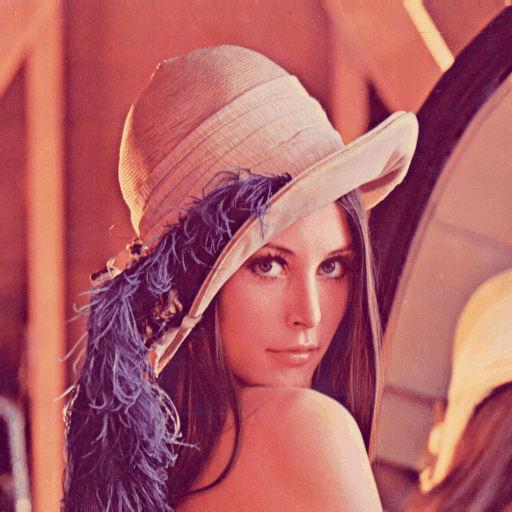
\includegraphics[width=\textwidth]{lena.png}
        \caption*{Originale}
      \end{subfigure}
      \hspace{0.15\textwidth}
      \begin{subfigure}[b]{0.33\textwidth}
        \centering
        
\includegraphics[width=\textwidth]{img/lena-threshold-20.png}
        \caption*{\texttt{p }\( = 20\%\)}
      \end{subfigure}

      \vspace{0.02\textwidth}

      \begin{subfigure}[b]{0.33\textwidth}
        \centering
        
\includegraphics[width=\textwidth]{img/lena-threshold-40.png}
        \caption*{\texttt{p }\( = 40\%\)}
      \end{subfigure}
      \hspace{0.15\textwidth}
      \begin{subfigure}[b]{0.33\textwidth}
        \centering
        
\includegraphics[width=\textwidth]{img/lena-threshold-60.png}
        \caption*{\texttt{p }\( = 60\%\)}
      \end{subfigure}

      \vspace{0.02\textwidth}

      \begin{subfigure}[b]{0.33\textwidth}
        \centering
        
\includegraphics[width=\textwidth]{img/lena-threshold-80.png}
        \caption*{\texttt{p }\( = 80\%\)}
      \end{subfigure}
      \hspace{0.15\textwidth}
      \begin{subfigure}[b]{0.33\textwidth}
        \centering
        
\includegraphics[width=\textwidth]{img/lena-threshold-99.png}
        \caption*{\texttt{p }\( = 99\%\)}
      \end{subfigure}
    \end{figure}

    È inoltre possibile creare, usando l'utility \texttt{convert} di
    ImageMagick, una gif animata i cui frame siano le immagini risultanti
    al variare della soglia da \(0\) a \(99\). Per ottenerla \`e sufficiente
    invocare la rule \texttt{make gif} del \texttt{Makefile} oppure visitare il
    seguente indirizzo: \href{http://raw.github.com/jacquerie/SPM/master/lena.gif}{\underline{http://raw.github.com/jacquerie/SPM/master/lena.gif}}.

  \newpage

  \appendix
    \section{Manuale d'uso}
      \subsection{Makefile}

      \begin{description}
	\item[\texttt{clean}:] Rimuove i file generati dalle rule \texttt{parallel}, \texttt{sequential} e \texttt{tex} eccetto \texttt{relazione.pdf}.
        \item[\texttt{gif}:] Genera una gif animata i cui frame sono le
          immagini risultanti al variare della soglia \texttt{p} da \(0\) a
          \(99\).
	\item[\texttt{nproc}:] Restituisce il numero di processori disponibili nel
	  \texttt{Machinefile}.
        \item[\texttt{parallel}:] Compila con \texttt{sketocxx}
          l'implementazione parallela.
  	\item[\texttt{pdf}:] Compila con \texttt{pdflatex} il presente
	  documento.
        \item[\texttt{sequential}:] Compila con \texttt{g++} l'implementazione
          sequenziale.
      \end{description}

      \subsection{Eseguibili}

      \begin{description}
	\item[\texttt{bin/generateMachinefile}:] Genera tramite \texttt{ping} e
	  connessioni ssh un \texttt{Machinefile} delle macchine funzionanti in
	  aula 4.
        \item[\texttt{bin/sequential numberOfJobs}:] Esegue l'implementazione
	  sequenziale su \texttt{numberOfJobs} istanze del problema dell'Histogram
          Thresholding. Stampa su \texttt{stdout} una coppia separata da uno
          spazio in cui il primo numero \`e \texttt{numberOfJobs} e il secondo
          il tempo in secondi impiegato da \texttt{bin/sequential} a meno di
          operazioni di lettura e scrittura sul file system. 
	\item[\texttt{bin/sequentialCluster}:] Script usato nella generazione
	  dei dati dell'implementazione sequenziale su una macchina dell'aula 4.
	\item[\texttt{bin/sequentialMulticore}:] Script usato nella generazione
	  dei dati dell'implementazione sequenziale su \texttt{andromeda.di.unipi.it}.
	\item[\texttt{bin/parallel}:] Binario contenente l'implementazione parallela
	  della soluzione al problema dell'Histogram Thresholding. Richiede di essere
	  invocato tramite \texttt{sketorun}.
	\item[\texttt{bin/parallelCluster}:] Script usato nella generazione dei
	  dei dati dell'implementazione parallela sulle macchine disponibili in aula 4.
	\item[\texttt{bin/parallelMulticore}:] Script usato nella generazione dei
	  dati dell'implementazione parallela su \texttt{andromeda.di.unipi.it}.
      \end{description}

      \subsection{Licenza}

      Il codice \`e rilasciato con \href{http://opensource.org/licenses/MIT}{\underline{licenza MIT}}
      ed \`e disponibile su \href{https://github.com/jacquerie/SPM}{\underline{Github}}.
\end{document}

